%% Chapter 2 — Formation.
%%
%% Premise: it behaves like an assistant because people rated outputs and it was optimised
%% toward those ratings.
%%
%% Rebuilt 2026-08-20 against curriculum/review-ch02.md. Four decisions drive the shape:
%%
%%   1. WOVEN, not split into 2a/2b. The split existed partly so a reader could tell which of
%%      two evidence bases a slide sat on - published papers, or five uncitable annotation
%%      instruments. The footer ruling dissolves that reason: every frame now declares its
%%      provenance, and \provenance{instrument} carries the document count. Nine of the ten
%%      taught findings have a natural host in the mechanism narrative, so each stage of the
%%      pipeline is followed immediately by what that stage looks like from inside the rating
%%      seat. THIS IS THE ONE STRUCTURAL CHOICE MADE WITHOUT A RULING. Overrule it freely.
%%   2. The order follows the pipeline diagram, in order, once.
%%   3. One running example: "What does lowering the water/cement ratio do to compressive
%%      strength?" - the same question Chapter 1's opening figure asks, in the shared domain,
%%      with an answer the room can check cold.
%%   4. The phenomenon before the explanation: the pretrained model is shown failing to answer
%%      before anything is said about what was added.
%%
%% CLAUDE.md rule 5 governs every example here: nothing is reproduced or paraphrased from any
%% source document. Every instrument, rubric and response is synthetic and built on mechanics,
%% concrete and fluids. Documents are referred to by count only.
\documentclass[aspectratio=169,11pt]{beamer}
\usetheme{UHTraining}
%% Shared preamble for the course decks.
\usepackage{uhcite}
\usepackage{uhslot}
\usepackage{amsmath}
\usetikzlibrary{arrows.meta,positioning}

%% --- the four kinds of number ------------------------------------------------
%% A review found parameters, token IDs, logits and probabilities were all appearing as
%% bare numbers with nothing telling them apart. Each now has one colour, used identically
%% in the slides, the figures and the animations. Colour is a redundant cue: every coloured
%% number carries its word too, so nothing depends on hue alone.
\newcommand{\tokid}[1]{\textcolor{uhslate}{\textbf{#1}}}   % a label, no magnitude
\newcommand{\param}[1]{\textcolor{uhocher}{\textbf{#1}}}   % the fitted numbers
\newcommand{\logit}[1]{\textcolor{uhteal}{\textbf{#1}}}    % raw scores out of the network
\newcommand{\prob}[1]{\textcolor{uhred}{\textbf{#1}}}      % probabilities
%% Defined terms are bold and black. Colour is reserved for number kinds, so that a colour
%% on a slide always answers the same question: what sort of number is this?
\newcommand{\kw}[1]{\textbf{#1}}
%% Inside an equation the same colours apply without \textbf, which is text-mode and breaks
%% on a subscript. Colour only; maths keeps its own italic.
\newcommand{\mlogit}[1]{\textcolor{uhteal}{#1}}
\newcommand{\mprob}[1]{\textcolor{uhred}{#1}}

%% --- a figure that an animation replaces in the PowerPoint version ------------
\newcommand{\animatable}[2]{%
  \vspace{-0.5em}{\scriptsize\color{uhocher}\textbf{animation #1} replaces this figure --- #2}\par}

%% --- diagram styles ----------------------------------------------------------
\tikzset{
  uhbox/.style   ={draw=uhslate!70, fill=uhslate!7,  rounded corners=1pt, align=center,
                   font=\scriptsize, inner sep=3pt, minimum height=8mm, text width=19mm},
  uhwide/.style  ={uhbox, text width=26mm},
  uhhi/.style    ={uhbox, draw=uhred, fill=uhred!8, thick},
  uhamber/.style ={uhbox, draw=uhocher, fill=uhocher!12, thick},
  uhghost/.style ={uhbox, draw=uhslate!45, fill=none, dashed},
  uhar/.style    ={-{Latex[length=1.8mm]}, draw=uhslate!80, thick},
  uhardot/.style ={-{Latex[length=1.8mm]}, draw=uhslate!55, thick, dashed},
}

% Generated from references.md by gen-sources-tex.mjs. Do not edit by hand.
\uhdefsource{vaswani2017}{V}{Vaswani, A., Shazeer, N., Parmar, N., Uszkoreit, J., Jones, L., Gomez, A. N., Kaiser, L. \& Polosukhin, I., 2017. \emph{Attention Is All You Need}, arXiv:1706.03762.}{}
\uhdefsource{anthropic-code-exec}{V}{Anthropic, 2026. \emph{Code execution tool, platform.claude.com --- vendor documentation, fetched 2026-08-20}.}{}
\uhdefsource{kaplan2020}{V}{Kaplan, J., McCandlish, S., Henighan, T., et al., 2020. \emph{preprint}, arXiv:2001.08361.}{}
\uhdefsource{hoffmann2022}{V}{Hoffmann, J., Borgeaud, S., Mensch, A., et al., 2022. \emph{preprint --- venue unconfirmed}, arXiv:2203.15556.}{}
\uhdefsource{fedus2021}{V}{Fedus, W., Zoph, B. \& Shazeer, N., 2021. \emph{arXiv preprint; version of record JMLR 23(120):1--39, 2022}, arXiv:2101.03961.}{}
\uhdefsource{lepikhin2020}{V}{Lepikhin, D., Lee, H., Xu, Y., et al., 2020. \emph{arXiv preprint; ICLR 2021}, arXiv:2006.16668.}{}
\uhdefsource{clark2022}{V}{Clark, A., de las Casas, D., Guy, A., et al., 2022. \emph{ICML 2022, pp. 4057--4086}, arXiv:2202.01169.}{}
\uhdefsource{stiennon2020}{V}{Stiennon, N., Ouyang, L., Wu, J., et al., 2020. \emph{preprint --- venue unconfirmed}, arXiv:2009.01325.}{}
\uhdefsource{ouyang2022}{V}{Ouyang, L., Wu, J., Jiang, X., et al., 2022. \emph{NeurIPS 2022}, arXiv:2203.02155.}{}
\uhdefsource{bai2022hh}{V}{Bai, Y., Jones, A., Ndousse, K., et al., 2022. \emph{preprint}, arXiv:2204.05862.}{}
\uhdefsource{bai2022cai}{V}{Bai, Y., Kadavath, S., Kundu, S., et al., 2022. \emph{preprint}, arXiv:2212.08073.}{}
\uhdefsource{rafailov2023}{V}{Rafailov, R., Sharma, A., Mitchell, E., Ermon, S., Manning, C. D. \& Finn, C., 2023. \emph{NeurIPS 2023}, arXiv:2305.18290.}{}
\uhdefsource{ye2024}{V}{Ye, Q., Axmed, M., Pryzant, R. \& Khani, F., 2024. \emph{Findings of the ACL 2024}, arXiv:2311.05661.}{}
\uhdefsource{li2023emotion}{V}{Li, C., Wang, J., Zhang, Y., et al., 2023. \emph{technical report, not peer reviewed}, arXiv:2307.11760.}{}
\uhdefsource{vaugrante2024}{V}{Vaugrante, L., Niepert, M. \& Hagendorff, T., 2024. \emph{preprint --- venue unconfirmed}, arXiv:2409.20303.}{}
\uhdefsource{yang2023}{V}{Yang et al., 2023. \emph{Google DeepMind; arXiv preprint (ICLR 2024 per the arXiv comment)}, arXiv:2309.03409.}{}
\uhdefsource{wei2022}{V}{Wei, J., Wang, X., Schuurmans, D., Bosma, M., Ichter, B., Xia, F., Chi, E., Le, Q. \& Zhou, D., 2022. \emph{Chain-of-Thought Prompting Elicits Reasoning in Large Language Models}, arXiv:2201.11903.}{}
\uhdefsource{anthropic-prompting}{V}{Anthropic, 2026. \emph{Prompting best practices, platform.claude.com --- vendor documentation, fetched 2026-08-19}.}{}
\uhdefsource{anthropic-models}{V}{Anthropic, 2026. \emph{Models overview, platform.claude.com --- vendor documentation, fetched 2026-08-20}.}{}
\uhdefsource{anthropic-thinking}{V}{Anthropic, 2026. \emph{Steering thinking, platform.claude.com --- vendor documentation, fetched 2026-08-20}.}{}
\uhdefsource{erratum2026}{V}{Reader comment (unattributed), 2026. \emph{Comment thread on the Pope lecture transcript gist --- reader correction, not a primary result}.}{testimony}
\uhdefsource{zheng2024}{V}{Zheng, M., Pei, J., Logeswaran, L., Lee, M. \& Jurgens, D., 2024. \emph{Findings of the ACL: EMNLP 2024, pp. 15126--15154}, DOI 10.18653/v1/2024.findings-emnlp.888.}{}
\uhdefsource{liu2024}{V}{Liu, N. F., Lin, K., Hewitt, J., Paranjape, A., Bevilacqua, M., Petroni, F. \& Liang, P., 2024. \emph{Transactions of the ACL 12, pp. 157--173}, DOI 10.1162/tacl\_a\_00638.}{}
\uhdefsource{velickovic2025}{V}{Veličković, P., Perivolaropoulos, C., Barbero, F. \& Pascanu, R., 2025. \emph{ICML 2025, PMLR 267, pp. 61190--61211}, arXiv:2410.01104.}{}
\uhdefsource{kamradt2023}{V}{Kamradt, G., 2023. \emph{Needle in a Haystack --- software implementation, not a peer-reviewed result}, github.com/gkamradt/needle-in-a-haystack.}{}
\uhdefsource{chroma2025}{V}{Hong, K., Troynikov, A. \& Huber, J., 2025. \emph{Chroma technical report --- COI, see below}, trychroma.com/research/context-rot.}{coi}
\uhdefsource{liang2023}{V}{Liang, W., Yuksekgonul, M., Mao, Y., Wu, E. \& Zou, J., 2023. \emph{Patterns 4(7):100779}, DOI 10.1016/j.patter.2023.100779.}{}
\uhdefsource{dathathri2024}{V}{Dathathri, S., See, A., Ghaisas, S., et al., 2024. \emph{Nature 634(8035), pp. 818--823}, DOI 10.1038/s41586-024-08025-4.}{}
\uhdefsource{bricken2023}{V}{Bricken, T., Templeton, A., Batson, J., et al., 2023. \emph{Anthropic, Transformer Circuits Thread --- COI, lab publishing on its own models}, transformer-circuits.pub.}{coi}
\uhdefsource{templeton2024}{V}{Templeton, A., Conerly, T., Marcus, J., et al., 2024. \emph{Anthropic, Transformer Circuits Thread --- COI, lab publishing on its own models}, arXiv:2605.29358.}{coi}
\uhdefsource{ameisen2025}{V}{Ameisen, E., Lindsey, J., Pearce, A., et al., 2025. \emph{Anthropic, Transformer Circuits Thread --- COI, lab publishing on its own models}, transformer-circuits.pub.}{coi}
\uhdefsource{lindsey2025}{V}{Lindsey, J., Gurnee, W., Ameisen, E., et al., 2025. \emph{Anthropic, Transformer Circuits Thread --- COI, lab publishing on its own models}, transformer-circuits.pub.}{coi}
\uhdefsource{turpin2023}{V}{Turpin, M., Michael, J., Perez, E. \& Bowman, S. R., 2023. \emph{NeurIPS 2023}, arXiv:2305.04388.}{}
\uhdefsource{chen2025}{V}{Chen, Y., Benton, J., Radhakrishnan, A., et al., 2025. \emph{Anthropic --- COI, lab publishing on its own models}, arXiv:2505.05410.}{coi}
\uhdefsource{greshake2023}{V}{Greshake, K., Abdelnabi, S., Mishra, S., Endres, C., Holz, T. \& Fritz, M., 2023. \emph{AISec '23, pp. 79--90}, DOI 10.1145/3605764.3623985.}{}
\uhdefsource{owasp2026}{V}{OWASP GenAI Security Project, 2026. \emph{OWASP Top 10 for LLM Applications, 2026 edition}, LLM01:2026.}{}
\uhdefsource{cohen2025}{V}{Cohen, S., Bitton, R. \& Nassi, B., 2025. \emph{ACM CCS 2025, pp. 3975--3989}, DOI 10.1145/3719027.3765196.}{}
\uhdefsource{aisi2026}{V}{UK AI Security Institute, 2026. \emph{Incident report, aisi.gov.uk --- blog page read; technical report not read}, INC-2026-07-28-01.}{}
\uhdefsource{pope2026}{V}{Pope, R., 2026. \emph{Dwarkesh Podcast, blackboard lecture; transcript published as a public gist}.}{testimony,coi}
\uhdefsource{revnets}{V}{Gomez, A. N., Ren, M., Urtasun, R. \& Grosse, R. B., 2017. \emph{The Reversible Residual Network: Backpropagation Without Storing Activations}, arXiv:1707.04585.}{}
\uhdefsource{ornes2025}{V}{Ornes, S., 2025. \emph{PNAS 122(44) --- secondary account, not primary research}, DOI 10.1073/pnas.2528654122.}{}
\uhdefsource{smirnova2023}{V}{Smirnova, L., Caffo, B. S., Gracias, D. H., et al., 2023. \emph{Frontiers in Science 1}, DOI 10.3389/fsci.2023.1017235.}{}
\uhdefsource{schrimpf2021}{V}{Schrimpf, M., Blank, I. A., Tuckute, G., et al., 2021. \emph{PNAS 118(45):e2105646118}, DOI 10.1073/pnas.2105646118.}{}
\uhdefsource{goldstein2022}{V}{Goldstein, A., Zada, Z., Buchnik, E., et al., 2022. \emph{Nature Neuroscience 25(3):369--380}, DOI 10.1038/s41593-022-01026-4.}{}
\uhdefsource{antonello2024}{V}{Antonello, R. \& Huth, A., 2024. \emph{Neurobiology of Language 5(1):64--79}, DOI 10.1162/nol\_a\_00087.}{}
\uhdefsource{hadidi2026}{V}{Hadidi, N., Feghhi, E., Song, B. H., Blank, I. A. \& Kao, J. C., 2026. \emph{Nature Communications 17(1):5769}, DOI 10.1038/s41467-026-72253-7.}{}
\uhdefsource{fedorenko2024}{V}{Fedorenko, E., Piantadosi, S. T. \& Gibson, E. A. F., 2024. \emph{Nature 630(8017)}, DOI 10.1038/s41586-024-07522-w.}{}
\uhdefsource{diachek2020}{V}{Diachek, E., Blank, I., Siegelman, M., Affourtit, J. \& Fedorenko, E., 2020. \emph{Journal of Neuroscience 40(23):4536--4550}, DOI 10.1523/JNEUROSCI.2036-19.2020.}{}
\uhdefsource{cowan2001}{V}{Cowan, N., 2001. \emph{Behavioral and Brain Sciences 24(1):87--114, discussion 114--185}, DOI 10.1017/S0140525X01003922.}{}
\uhdefsource{claudecode-docs}{V}{Anthropic, 2026. \emph{Claude Code documentation, code.claude.com --- vendor documentation, version-dependent}.}{}
\uhdefsource{anthropic-support}{V}{Anthropic, 2026. \emph{Anthropic support centre, support.claude.com --- vendor documentation, version-dependent}.}{}
\uhdefsource{graphify}{V}{Graphify project, 2026. \emph{graphify 0.9.16, behaviour observed directly on this machine 2026-08-19}, version 0.9.16.}{}
\uhdefsource{mcp-spec}{V}{Model Context Protocol, 2025-06-18. \emph{modelcontextprotocol.io --- protocol specification}, version 2025-06-18.}{}
\uhdefsource{anthropic-pdf}{V}{Anthropic, 2026. \emph{PDF support, platform.claude.com --- vendor documentation, fetched 2026-08-20}.}{}


\courseflowreset
\courseflowstep{Substrate}{}
\courseflowstep{Formation}{}
\courseflowstep{Control}{}
\courseflowstep{Measure}{}
\courseflowstep{Failure}{}
\courseflowstep{Limits}{}
\courseflowcurrent{2}
\uhshorttitle{Chapter 2 --- Formation}

\title{Chapter 2 --- Formation}
\subtitle{How a predictor became an assistant}
\author{AI Training}
\institute{University of Houston}
\date{2026}

\graphicspath{{../../assets/figures/}}

%% The running question, so it is written once and cannot drift between frames.
\newcommand{\runq}{\emph{What does lowering the water/cement ratio do to compressive strength?}}

\begin{document}

% ---------------------------------------------------------------- 1
\begin{frame}[plain]
  \titlepage
  \provenance{none}
\end{frame}
\note{%
Chapter 1 closed on a question: nothing in scoring text fragments makes a thing that answers a
question, follows an instruction, or declines a request. This chapter answers it.}

% ---------------------------------------------------------------- 2
\begin{frame}{A model that only scores text continues your question instead of answering it}
  \slotF{the running question typed into a model that has had nothing added --- it continues with more questions}

  {\small The question, throughout this chapter: \runq}
  \provenance{observation}
\end{frame}
\note{%
The phenomenon before the explanation. Do not say what was added until the room has seen what is
missing.\\[0.3em]
What a pretrained model does with a question is continue the document it looks like it came from.
A page with a question on it is usually followed by more questions, so that is what comes back.
Every attendee will recognise it as wrong, and none of them will be able to say why the tool they
actually use behaves differently. That gap is the chapter.\\[0.3em]
TODO(capture): a base model, not an instruction-tuned one, given the running question. Record the
model ID and the date. If no base model is reachable, a documented transcript is acceptable, and
the slide must say which it is.}

% ---------------------------------------------------------------- 3
\begin{frame}{Four stages turn a predictor into something that answers}
  \begin{center}
  \begin{tikzpicture}[node distance=6mm]
    \node[uhwide]                  (a) {a very large\\corpus};
    \node[uhhi, right=of a]        (b) {pretraining};
    \node[uhwide, right=of b]      (c) {demonstrations\\written by people};
    \node[uhamber, right=of c]     (d) {preferences\\expressed by people};
    \node[uhwide, right=of d]      (e) {a model of\\a rater};
    \node[uhbox, right=of e]       (f) {optimise\\against it};
    \draw[uhar] (a)--(b); \draw[uhar] (b)--(c); \draw[uhar] (c)--(d);
    \draw[uhar] (d)--(e); \draw[uhar] (e)--(f);
  \end{tikzpicture}
  \end{center}
  {\small Every stage after the first is a person's judgement, written down and turned into a
   number. \kw{Each name on this diagram is defined on the frame that expands it}, and the chapter
   walks the diagram once, left to right, stopping at each stage to ask what the job actually
   looks like.}
  \provenance{derived}
\end{frame}
\note{%
The map. Say plainly that we follow it in order and do not jump about.\\[0.3em]
The three additions are demonstrations, preferences, and optimisation against a model of those
preferences. Naming them here means every later frame has somewhere to attach.\\[0.3em]
The stages are not equally expensive or equally understood. Pretraining is the one with the
published scaling results; the rating layer is the one nobody outside it describes, and it is where
this chapter spends most of its time.}

% ---------------------------------------------------------------- 4
\begin{frame}{Pretraining runs one objective over a very large corpus, and then it stops}
  \begin{center}
  \begin{tikzpicture}[node distance=7mm]
    \node[uhwide]                    (a) {text, at a scale\\nobody reads};
    \node[uhhi, right=of a]          (b) {predict the\\next token};
    \node[uhwide, right=of b]        (c) {\param{parameters}\\adjusted};
    \node[uhamber, right=14mm of c]  (d) {a very good\\autocomplete};
    \draw[uhar] (a)--(b); \draw[uhar] (b)--(c);
    \draw[uhar] (c) -- node[above,font=\scriptsize\itshape]{it ends} (d);
    \draw[uhar] (c.south) -- ++(0,-6mm) -| node[pos=0.25,below,font=\scriptsize\itshape]
      {repeat over the corpus} (b.south);
  \end{tikzpicture}
  \end{center}
  \begin{columns}[t]
    \begin{column}{0.31\linewidth}\centering
      \kw{No labels}\\[0.2em]{\small the text supervises itself, which is why the corpus could be so large}
    \end{column}
    \begin{column}{0.31\linewidth}\centering
      \kw{Knowledge cutoff}\\[0.2em]{\small the date it stopped, and a consequence rather than a policy}
    \end{column}
    \begin{column}{0.31\linewidth}\centering
      \kw{The corpus decides}\\[0.2em]{\small where it is strong, and where it is not}
    \end{column}
  \end{columns}
  \provenance{derived}
\end{frame}
\note{%
Chapter 1 defined training, inference and the cutoff. This frame adds only what is specific to
pretraining: no labels, no task, no supervision beyond the text itself.\\[0.3em]
What comes out is the thing on the previous frame. It is a very good autocomplete and it is not an
assistant.\\[0.3em]
Worth one sentence if asked about scale: performance improves predictably with model size, data and
compute, and a later correction showed models had been undertrained relative to their size. Neither
result promised an assistant. They describe how a loss falls, not how behaviour changes.}

% ---------------------------------------------------------------- 5
\begin{frame}{People write the answer that should have come out, and the model is trained on the pair}
  \begin{center}
  \begin{tikzpicture}[node distance=8mm]
    \node[uhwide, text width=34mm]        (q) {\textbf{request}\\\footnotesize lowering the water/cement ratio, and compressive strength};
    \node[uhamber, right=of q, text width=30mm] (h) {\textbf{a person writes\\the response}};
    \node[uhwide, right=of h, text width=26mm]  (p) {the pair is\\stored};
    \node[uhhi, right=of p, text width=26mm]    (t) {trained on};
    \draw[uhar] (q)--(h); \draw[uhar] (h)--(p); \draw[uhar] (p)--(t);
  \end{tikzpicture}
  \end{center}
  \begin{columns}[t]
    \begin{column}{0.31\linewidth}\centering
      \kw{Supervised fine-tuning}\\[0.2em]{\small the model learns the \emph{shape} of an answer --- that a question gets answered}
    \end{column}
    \begin{column}{0.31\linewidth}\centering
      \kw{System prompt}\\[0.2em]{\small standing text placed before your message, which this stage trains it to treat as instruction}
    \end{column}
    \begin{column}{0.31\linewidth}\centering
      \kw{Cheap in data terms}\\[0.2em]{\small and it does most of the visible work of turning autocomplete into an assistant}
    \end{column}
  \end{columns}
  \citesource{ouyang2022}
\end{frame}
\note{%
The first thing added. Everything after this stage is about quality rather than about format.\\[0.3em]
Define \kw{system prompt} here, because Chapter 3 uses it from its second frame: a block of standing
text placed before your message, which the provider or the application writes, and which the model
is trained to treat as instruction rather than as content.\\[0.3em]
The person writing these responses is doing a job with a specification, and the next three frames
are what that specification contains. That is where this chapter stops being a summary of papers.}

% ---------------------------------------------------------------- 6
\begin{frame}{The person repairs the text as well as judging it, against a written specification}
  \begin{center}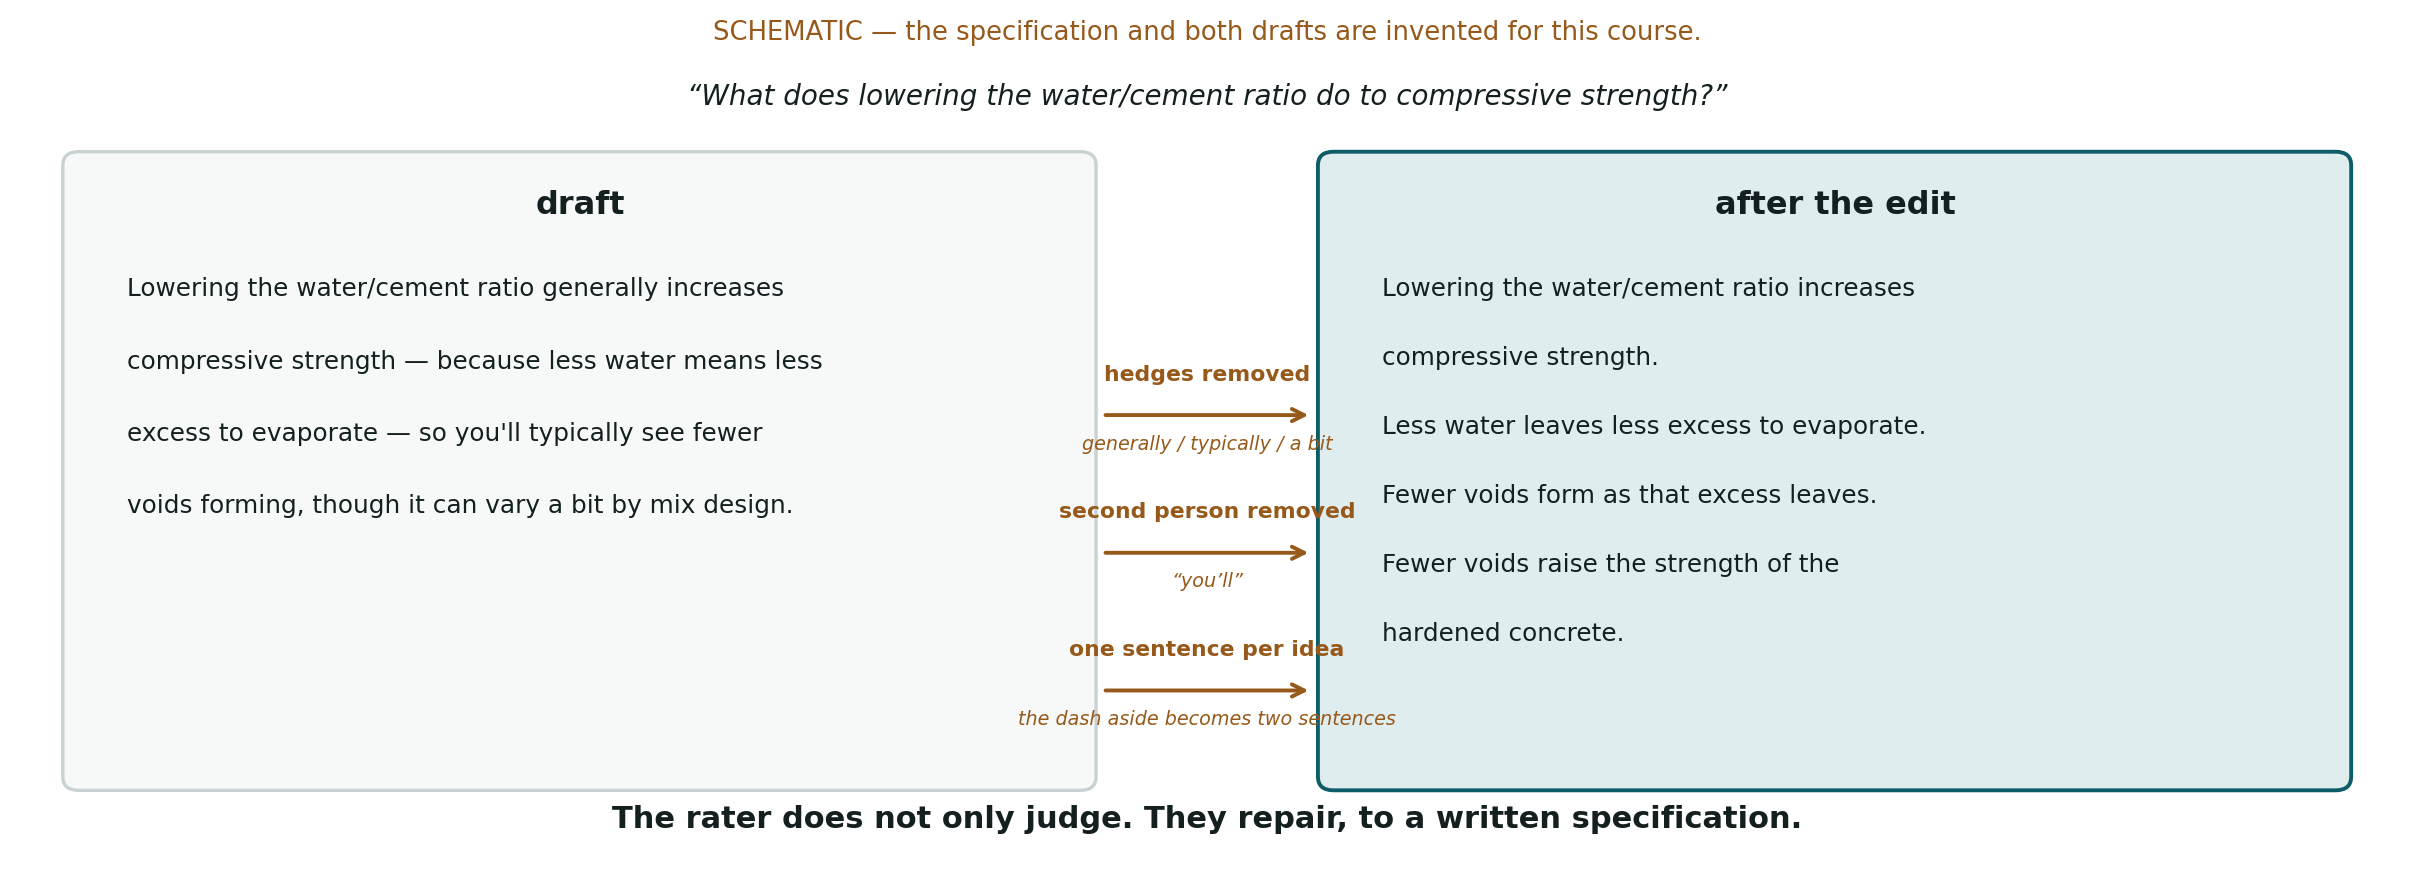
\includegraphics[height=32mm,width=\linewidth,keepaspectratio]{02-house-style}\end{center}
  {\small The person doing this is a \kw{rater} --- paid, working to a written instrument, usually
   with no contact with the people who wrote it. The specification is not about being right. It is
   about punctuation, hedging, person, sentence length and the shape of a list.}
  \provenance[Three of five documents.]{instrument}
\end{frame}
\note{%
The most concrete item in the whole set, and the reason to teach this chapter from inside the job
rather than from the outside.\\[0.3em]
Raters do not only pick A or B. They repair, to a written edit specification, and the specification
constrains prose down to the punctuation.\\[0.3em]
The example on the frame is invented for this course, on this room's domain. No worked example,
rubric row or banned-phrase list from any source document appears anywhere in this chapter. Say
that out loud if anyone asks where it came from.\\[0.3em]
This is where model voice comes from, and the next frame is the qualification that claim needs.}

% ---------------------------------------------------------------- 7
\begin{frame}{In two of the five instruments, the repaired text is what gets collected}
  \begin{center}
  \begin{tikzpicture}[node distance=7mm]
    \node[uhwide, text width=28mm]              (d) {the draft the\\model produced};
    \node[uhamber, right=of d, text width=28mm] (e) {the person's\\repaired version};
    \node[uhhi, right=of e, text width=30mm]    (c) {collected as\\training data};
    \node[uhghost, below=8mm of c, text width=30mm] (n) {or used only to sharpen\\the person's judgement};
    \draw[uhar] (d)--(e); \draw[uhar] (e)--(c);
    \draw[uhardot] (e.south) |- (n.west);
  \end{tikzpicture}
  \end{center}
  {\small The labour recurs in three documents. The repaired text entering the data is a separate
   claim on weaker evidence, and in one instrument the repaired version is explicitly not trained on.}
  \provenance[Two of five documents for collection; three of five for the labour.]{instrument}
\end{frame}
\note{%
Two claims were welded together in an earlier version of this material and they carry different
evidence. Separating them is the point of the frame.\\[0.3em]
The labour recurs: three of five documents have the human produce a target artefact rather than
only a verdict. Whether that artefact enters the training data is a narrower claim, resting on two.\\[0.3em]
Saying the weaker half is weaker is what makes the stronger half worth believing. This room will
test that habit against everything else in the course.}

% ---------------------------------------------------------------- 8
\begin{frame}{Demonstrations cannot cover everything, so preferences are collected instead}
  \begin{center}
  \begin{tikzpicture}[node distance=7mm]
    \node[uhwide, text width=30mm]              (q) {one request};
    \node[uhbox, right=of q, text width=24mm, yshift=7mm]  (a) {response A};
    \node[uhbox, right=of q, text width=24mm, yshift=-7mm] (b) {response B};
    \node[uhamber, right=32mm of q, text width=26mm]       (h) {a person\\chooses};
    \node[uhhi, right=of h, text width=26mm]               (n) {a comparison,\\stored};
    \draw[uhar] (q)--(a); \draw[uhar] (q)--(b);
    \draw[uhar] (a)--(h); \draw[uhar] (b)--(h); \draw[uhar] (h)--(n);
  \end{tikzpicture}
  \end{center}
  {\small Writing the ideal answer to every possible request is impossible. Judging which of two
   answers is better is not.}
  \citesource{stiennon2020}
\end{frame}
\note{%
The move that makes the rest of the pipeline possible, and the move that introduces everything
strange about the result.\\[0.3em]
A comparison is cheaper than a demonstration and it carries less information. What survives is an
ordering, not a reason.\\[0.3em]
The next six frames are what a comparison actually costs to produce, which is the part of this
pipeline that has no published description.}

% ---------------------------------------------------------------- 9
\begin{frame}{A rating task is a rubric whose dimensions conflict}
  \begin{center}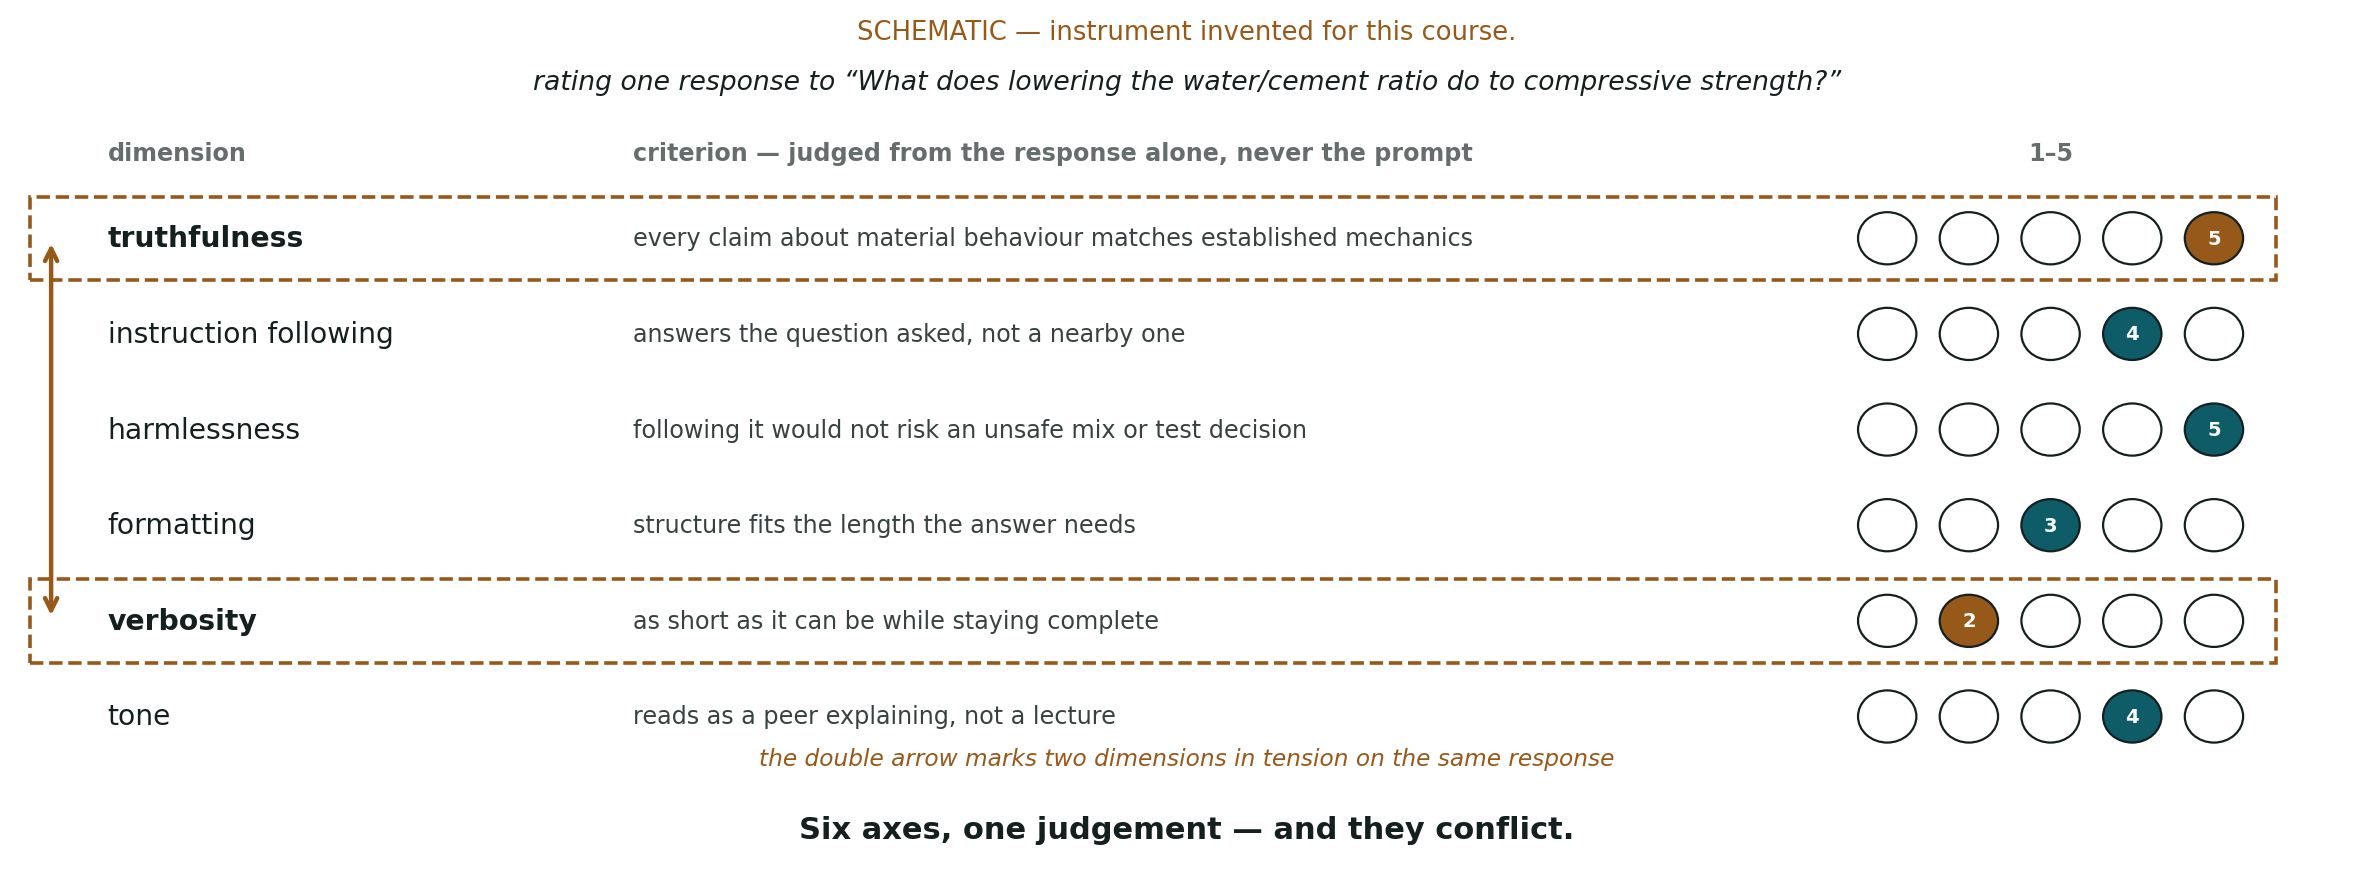
\includegraphics[height=36mm,width=\linewidth,keepaspectratio]{02-rubric}\end{center}
  {\small A response can be truthful and badly formatted, or fluent and wrong. Six axes, one
   judgement. \kw{Learn these six} --- each returns later in the course.}
  \provenance[The instrument shown is synthetic, built for this course.]{instrument}
\end{frame}
\note{%
These six dimensions are the spine of the rest of the course. Truthfulness becomes a structural
failure and then a work habit. Instruction following is what most of the next chapter steers.
Harmlessness becomes the trust boundary. Formatting is what wins when nobody in the room can check
the physics. Verbosity becomes a cost and then a bill. Tone is where house style lives.\\[0.3em]
Do not print the chapter numbers on the frame. Say them if asked.\\[0.3em]
The conflict is the content. A rater forced to produce one verdict from six axes is compressing,
and what survives the compression is what the reward model learns.}

% ---------------------------------------------------------------- 10
\begin{frame}{The person is made to attempt the task before judging it}
  \begin{center}
  \begin{tikzpicture}[node distance=7mm]
    \node[uhwide, text width=27mm]              (r) {read the request};
    \node[uhamber, right=of r, text width=30mm] (a) {\textbf{do the task}\\yourself, first};
    \node[uhwide, right=of a, text width=27mm]  (j) {then judge the\\two responses};
    \node[uhhi, right=of j, text width=27mm]    (v) {a verdict worth\\something};
    \draw[uhar] (r)--(a); \draw[uhar] (a)--(j); \draw[uhar] (j)--(v);
  \end{tikzpicture}
  \end{center}
  {\small The pipeline buys the attempt in order to get a reliable verdict. It is the most
   expensive step in the job and it is required in three of the five documents.}
  \provenance[Three of five documents.]{instrument}
\end{frame}
\note{%
Corrects the picture of an annotator idly picking A or B, and says something sharper than
"annotators work hard": the attempt is bought deliberately, because a verdict from someone who has
not tried the task is not worth collecting.\\[0.3em]
This room will recognise the principle. It is why you do not review a calculation you have not
attempted.}

% ---------------------------------------------------------------- 11
\begin{frame}{Verification is time-boxed at about fifteen minutes, against a ranked source list}
  \begin{center}
  \begin{tikzpicture}[node distance=6mm]
    \node[uhamber, text width=30mm]              (t) {about fifteen\\minutes, per task};
    \node[uhwide, right=10mm of t, text width=32mm, yshift=9mm]  (s1) {check the ranked\\sources first};
    \node[uhwide, right=10mm of t, text width=32mm]              (s2) {then anything\\else available};
    \node[uhhi, right=10mm of t, text width=32mm, yshift=-9mm]   (s3) {\textbf{or mark it\\unassessable}};
    \draw[uhar] (t)--(s1); \draw[uhar] (t)--(s2); \draw[uhar] (t)--(s3);
  \end{tikzpicture}
  \end{center}
  {\small A claim that would take longer than the box to check does not get checked. It gets a
   band of its own.}
  \provenance[One of five documents, stated as a rule.]{instrument}
\end{frame}
\note{%
The single most quotable item in the set for this audience, and the one they will think about
afterwards.\\[0.3em]
Say what it implies without overstating it: a fabricated citation in a response is exactly the kind
of claim that costs more than fifteen minutes to check. Under a time box it is marked unassessable
rather than false, which is the correct action under the instrument.\\[0.3em]
That is one document. Do not generalise it to the industry. It is enough that one pipeline is built
this way, because the room is about to do the same thing in the exercise and feel the pressure.}

% ---------------------------------------------------------------- 12
\begin{frame}{Two incompatible answers to who is qualified to judge}
  \begin{center}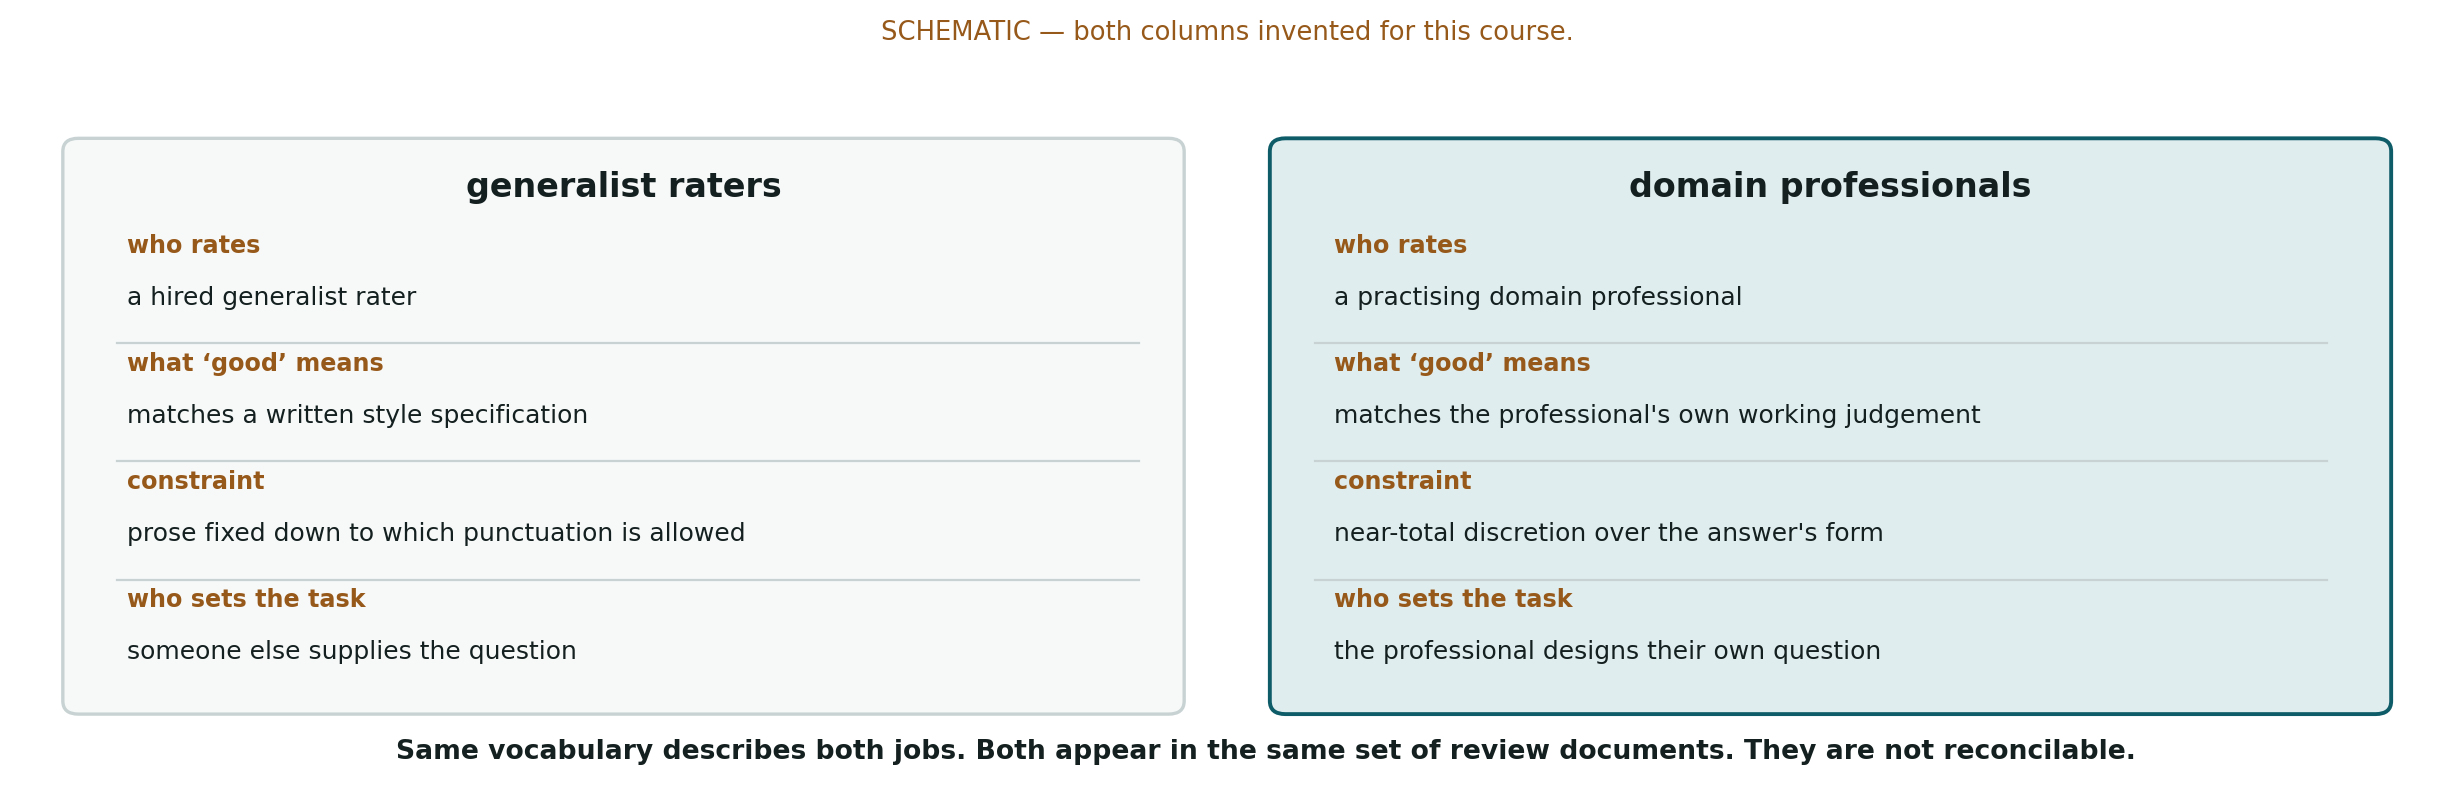
\includegraphics[height=36mm,width=\linewidth,keepaspectratio]{02-labour-models}\end{center}
  {\small Both are described with the same vocabulary. They are not the same job, and no single
   description of "the annotator" covers both.}
  \provenance[Corroborated across documents.]{instrument}
\end{frame}
\note{%
This frame dismantles the phrase "trained on human preferences" as a sentence that means anything
on its own. Which humans, doing which job, under which instrument?\\[0.3em]
It also lands harder on this audience than the alternative it partly replaced. An earlier version
of this material claimed vendors filter raters for English fluency; that rested on one document and
the defensible claim is narrower --- instruments impose English style rules on the prose they
collect. Say the narrower thing.}

% ---------------------------------------------------------------- 13
\begin{frame}{Equivalence is engineered out of the data, by opposite mechanisms}
  \begin{center}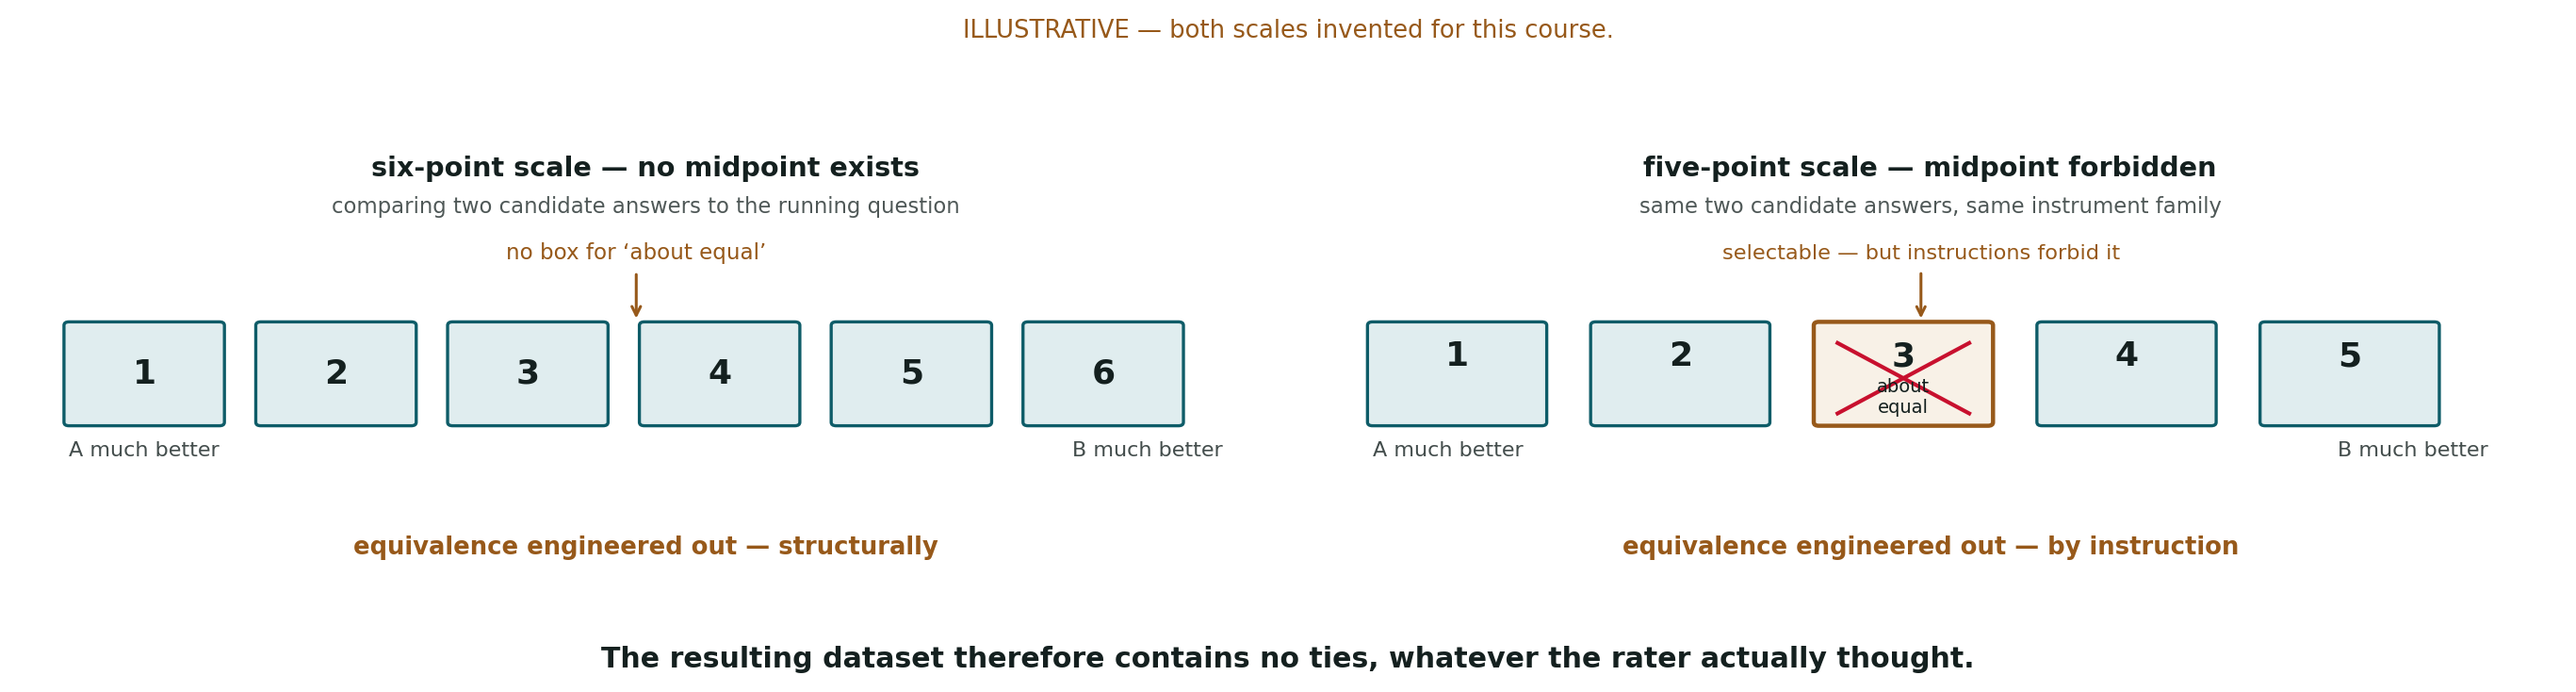
\includegraphics[height=38mm,width=\linewidth,keepaspectratio]{02-scale-designs}\end{center}
  {\small Two instruments, two opposite designs, the same result: the dataset contains no ties,
   whatever the rater actually thought.}
  \provenance[Two of five documents.]{instrument}
\end{frame}
\note{%
Two instruments arrive at the same place from opposite directions --- one removes the midpoint, the
other forbids using it. Convergent design is stronger evidence than either instrument alone.\\[0.3em]
What it reframes: a preference dataset is not a record of what people thought. It is a record of
what the instrument allowed them to say.\\[0.3em]
For a room of experimentalists this is a familiar failure. An instrument that cannot record a null
result produces a literature without null results.}

% ---------------------------------------------------------------- 14
\begin{frame}{One instrument collects comparisons only where a model has already failed}
  \begin{center}
  \begin{tikzpicture}[node distance=6mm]
    \node[uhwide, text width=30mm]                (t) {build a task};
    \node[uhamber, right=of t, text width=32mm]   (c) {does at least one\\response fail?};
    \node[uhhi, right=of c, text width=26mm]      (k) {keep it};
    \node[uhghost, below=8mm of c, text width=32mm] (d) {both good --- discard};
    \draw[uhar] (t)--(c);
    \draw[uhar] (c) -- node[above,font=\scriptsize]{yes} (k);
    \draw[uhardot] (c) -- node[right,font=\scriptsize,pos=0.35]{no} (d);
  \end{tikzpicture}
  \end{center}
  {\small The preference data from that instrument is conditioned on failure. It is not a sample of
   how the model behaves in use.}
  \provenance[One of five documents.]{instrument}
\end{frame}
\note{%
A selection effect, stated as a rule inside one instrument. This audience has a name for it and
will supply it before you do.\\[0.3em]
What it means downstream: the reward model is fitted on the cases where something went wrong, and
the distribution it was fitted on is not the distribution of ordinary use.\\[0.3em]
One document. Say so. It is the kind of design decision that would never appear in a paper about
the resulting model.}

% ---------------------------------------------------------------- 15
\begin{frame}{Realism in the data is manufactured to a specification}
  \begin{center}
  \begin{tikzpicture}[node distance=7mm]
    \node[uhwide, text width=32mm]                (s) {a written rule for\\what "realistic"\\means};
    \node[uhamber, right=of s, text width=32mm]   (w) {the contributor\\writes to it};
    \node[uhhi, right=of w, text width=34mm]      (d) {data that looks\\like it was captured\\from use};
    \draw[uhar] (s)--(w); \draw[uhar] (w)--(d);
  \end{tikzpicture}
  \end{center}
  {\small One line in one instrument, and it complicates the picture of preference data as
   behaviour observed in the wild.}
  \provenance[One of five documents.]{instrument}
\end{frame}
\note{%
Short frame, and it earns its place by what it removes rather than what it adds. The mental image
most people carry is of preference data captured from real usage. At least one pipeline manufactures
it to a specification for realism.\\[0.3em]
Do not overclaim. One line, one document. It is enough to make the room stop assuming.}

% ---------------------------------------------------------------- 16
\begin{frame}{One instrument was rebuilt in a single week, in the middle of collection}
  \begin{center}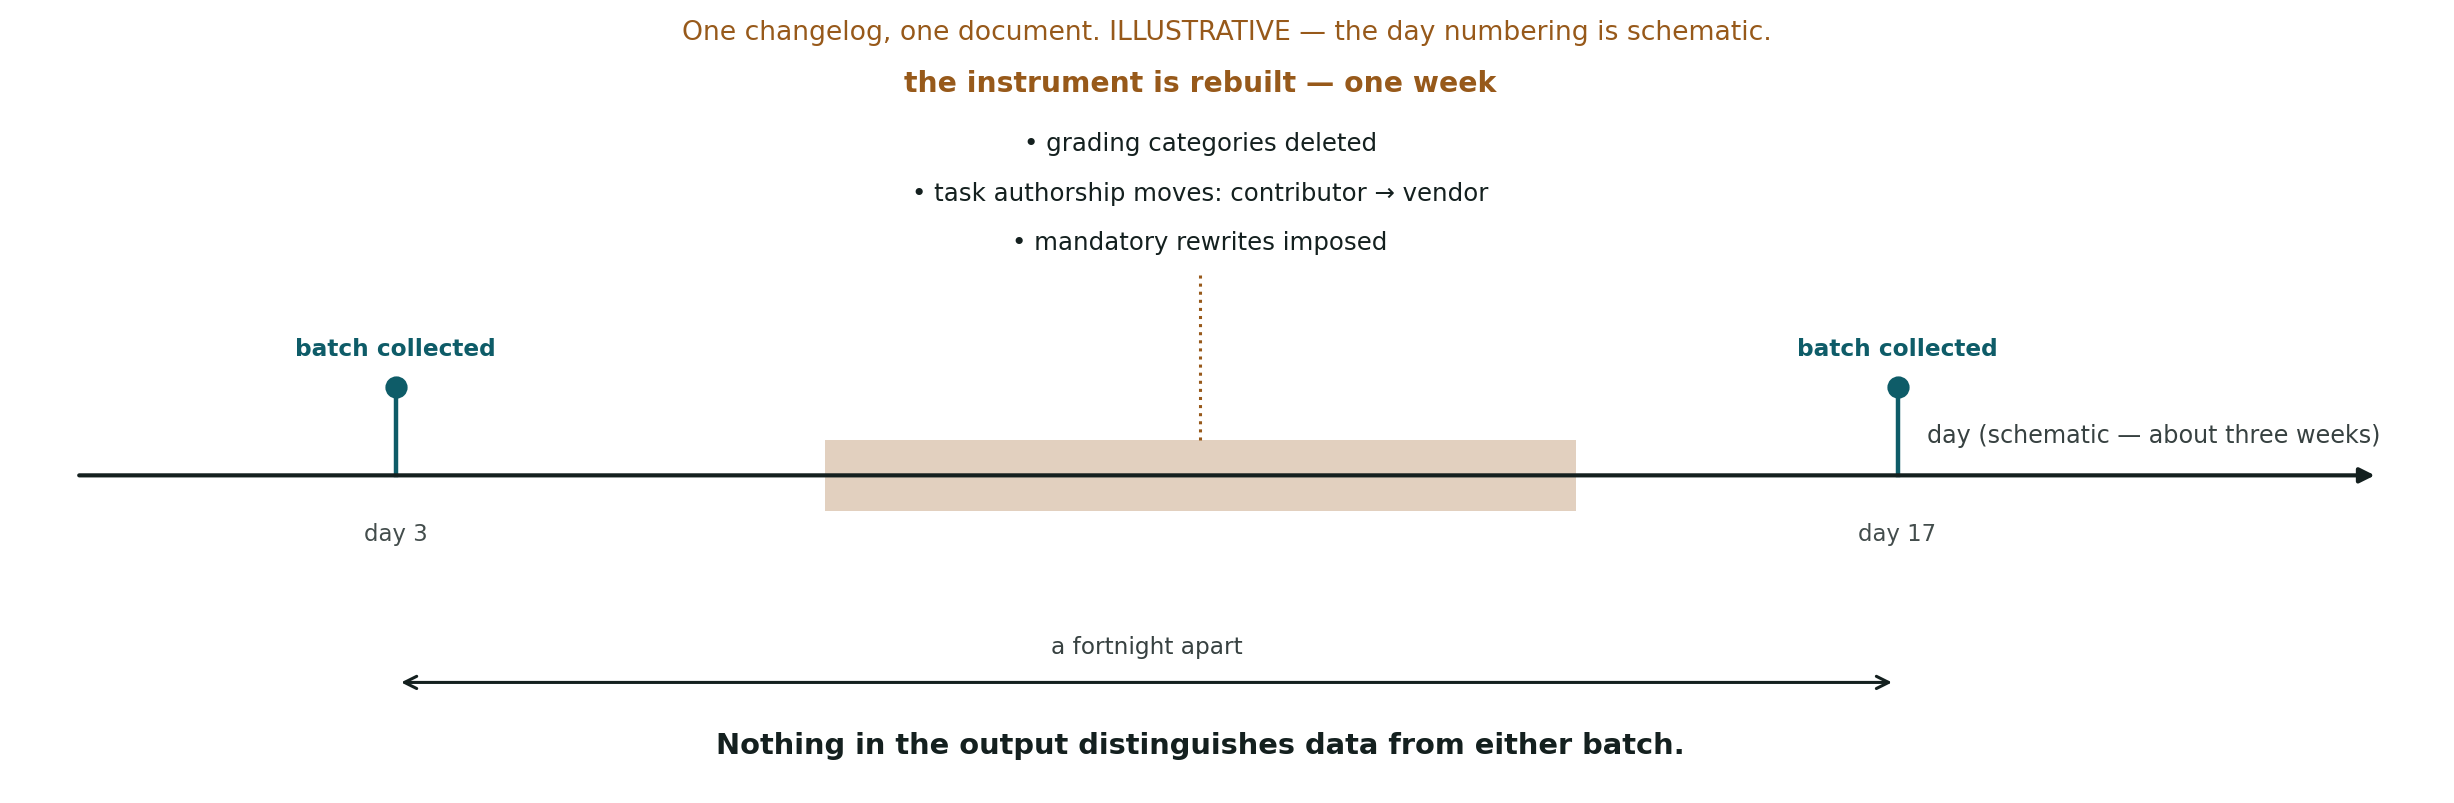
\includegraphics[height=36mm,width=\linewidth,keepaspectratio]{02-instrument-rebuild}\end{center}
  {\small Grading categories deleted, task authorship moved, mandatory rewrites imposed. Data
   gathered a fortnight apart was graded by materially different devices, with nothing in the
   output to distinguish them.}
  \provenance[One of five documents, from a dated changelog.]{instrument}
\end{frame}
\note{%
For a room of experimentalists this may be the most immediately persuasive item in the chapter.
It ranks eighth of fourteen by evidence, because it rests on one changelog.\\[0.3em]
Say both things, in that order. The gap between how forceful an item is and how well evidenced it
is, is itself the lesson, and the next frame but one makes it explicit.\\[0.3em]
The analogy that lands: a calibration drift nobody logged, in an instrument whose readings are
already in the dataset.}

% ---------------------------------------------------------------- 17
\begin{frame}{The instruments diverge in structure far more than in vocabulary}
  \begin{center}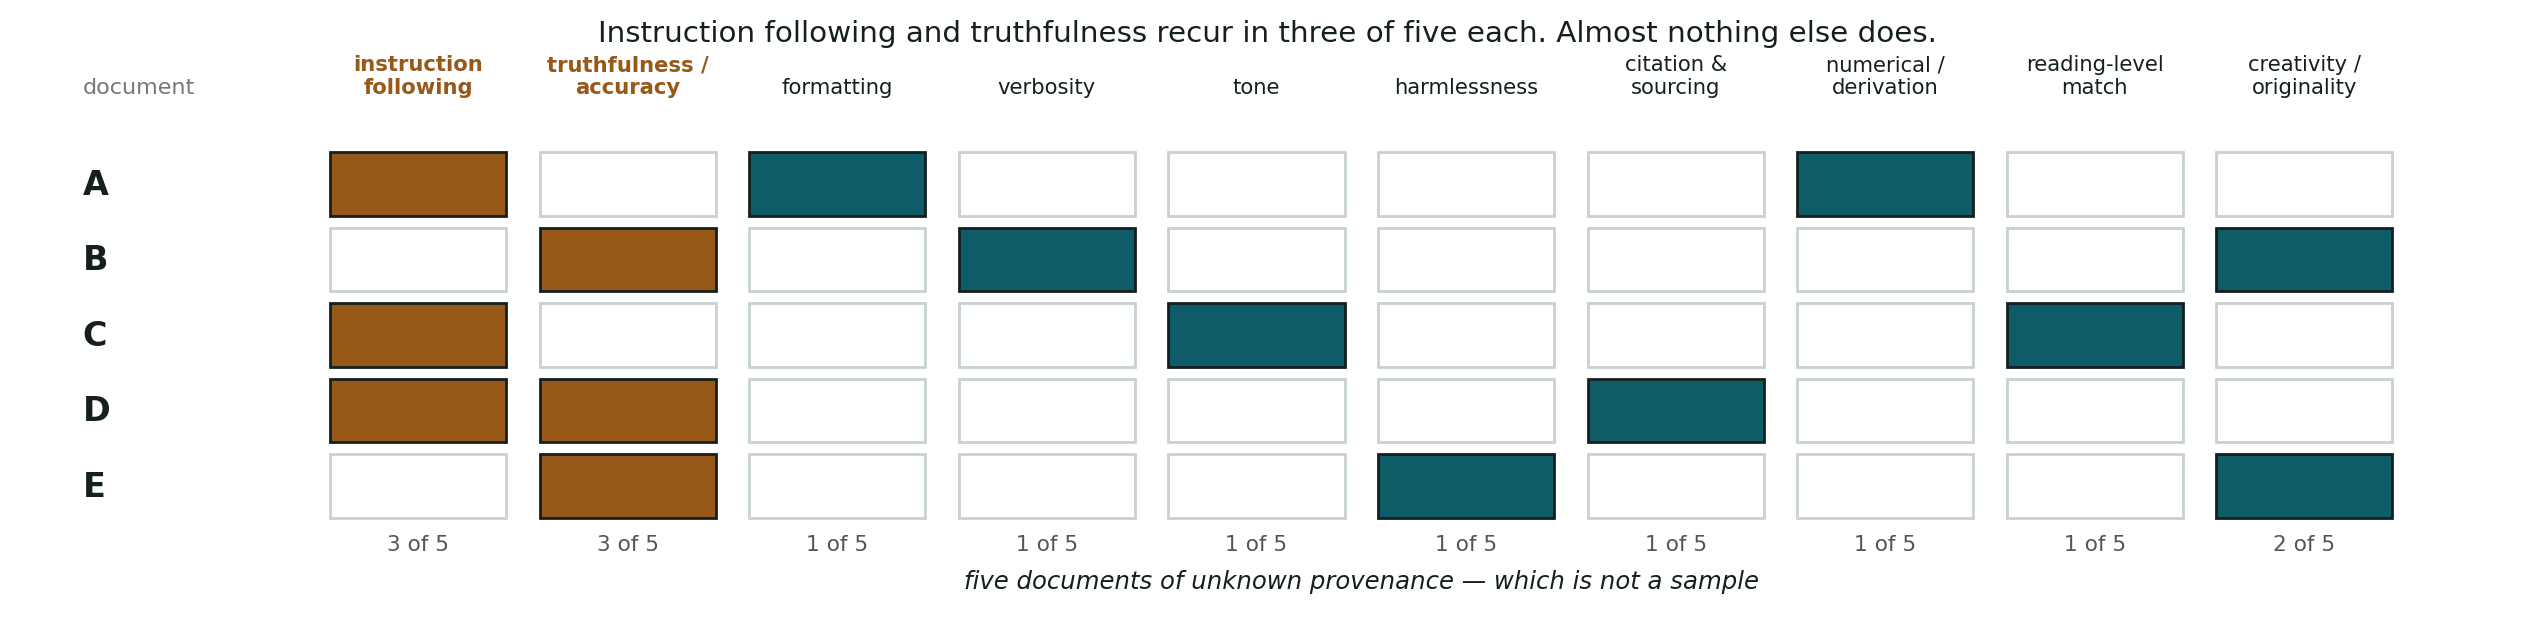
\includegraphics[height=36mm,width=\linewidth,keepaspectratio]{02-instrument-divergence}\end{center}
  {\small An instruction-following dimension recurs, and a truthfulness dimension recurs. Almost
   nothing else does --- not what else is measured, nor at what granularity, nor under what weighting.}
  \provenance[Five documents of unknown provenance, which is not a sample.]{instrument}
\end{frame}
\note{%
After this frame, "trained on human preferences" stops being a sentence that explains anything on
its own.\\[0.3em]
An earlier version of this material claimed the instruments shared almost no vocabulary. With five
documents that was too strong: there is partial convergence, and the divergence sits in the rest of
the instrument. The corrected claim is on the frame.\\[0.3em]
Two of the five were obtained as re-hosted copies, so their vendor, their client and their
completeness are unknown. Five documents are not a sample and this course does not present them as
one.}

% ---------------------------------------------------------------- 18
\begin{frame}{Two competent people disagree, and the disagreement goes into the data}
  \begin{center}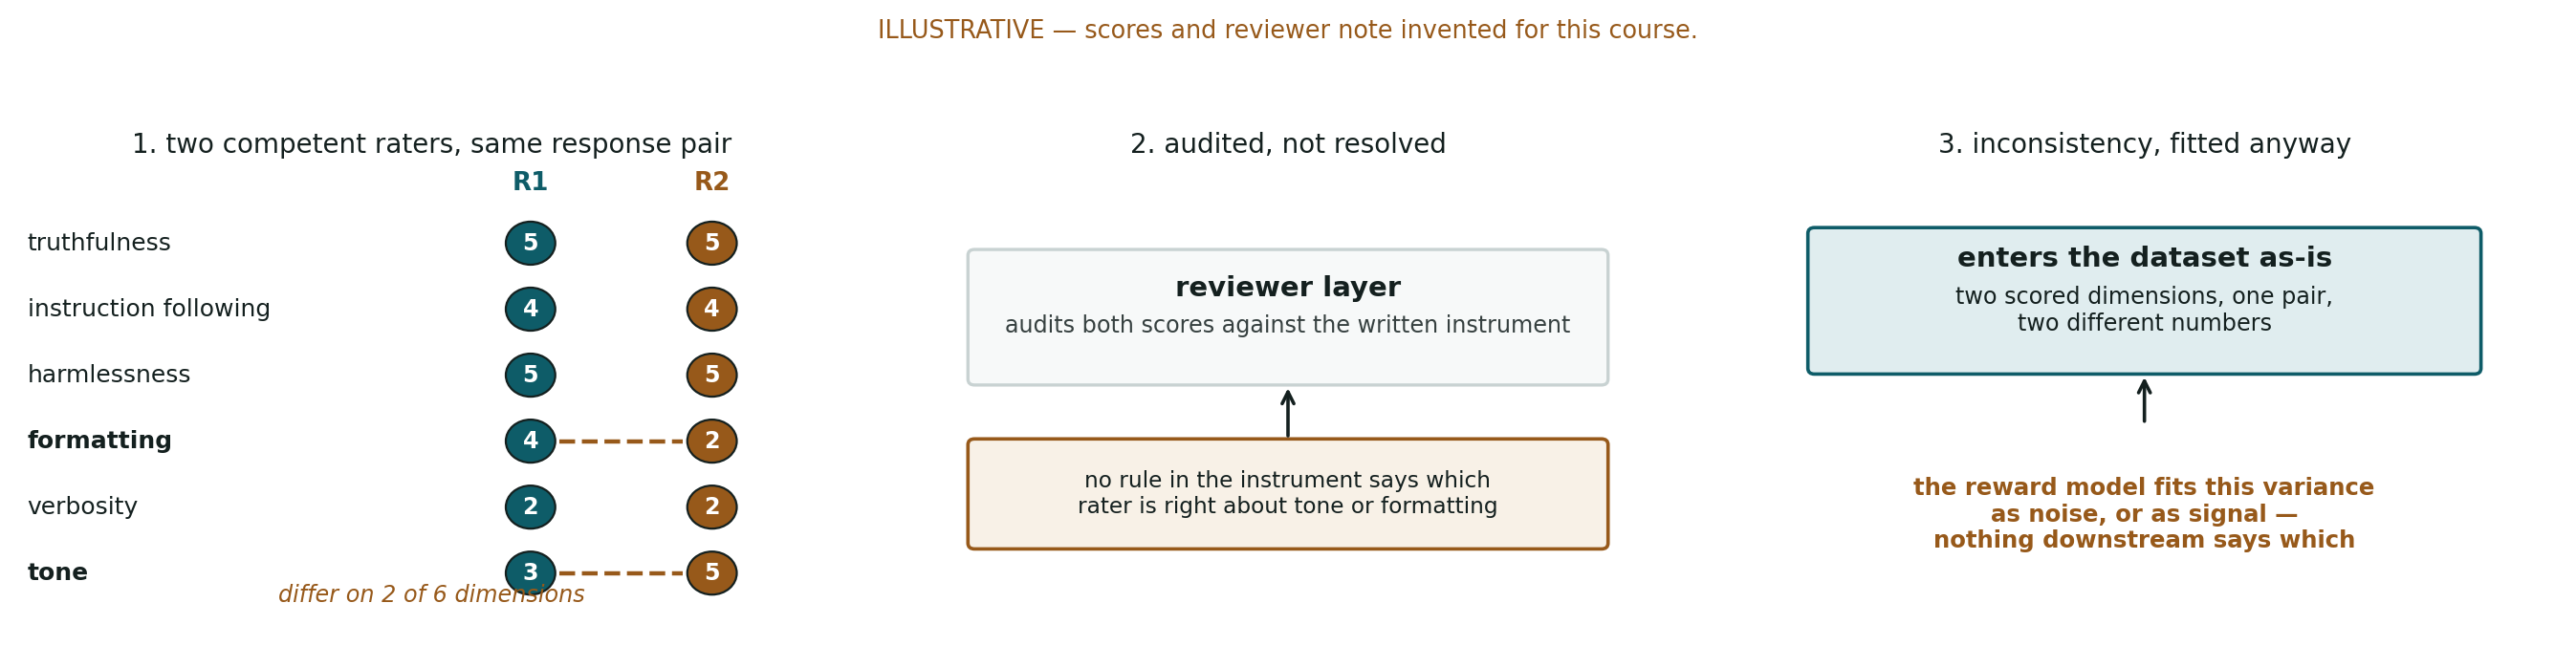
\includegraphics[height=36mm,width=\linewidth,keepaspectratio]{02-disagreement}\end{center}
  {\small Where they diverge, the question is whether the rubric or the rater is at fault. An
   ambiguous dimension produces disagreement that no amount of rater training removes.}
  \provenance[The audit layer is one of five documents; the downstream consequence is derived.]{instrument}
\end{frame}
\note{%
Disagreement is not noise to be eliminated. It is information, and what happens to it matters.\\[0.3em]
Unresolved disagreement does not vanish. It enters the preference data as inconsistency, and the
reward model on the next frame fits it along with everything else.\\[0.3em]
The room will occupy both sides of this in the exercise: rate, then audit somebody else's rating
against the same instrument.}

% ---------------------------------------------------------------- 19
\begin{frame}{The reward model is a model of a rater}
  \begin{center}
  \begin{tikzpicture}[node distance=7mm]
    \node[uhwide, text width=30mm]              (c) {comparisons made\\by particular people};
    \node[uhhi, right=of c, text width=28mm]    (r) {\textbf{a reward model}\\fitted to them};
    \node[uhamber, right=of r, text width=34mm] (s) {scores \emph{any} response,\\including ones no\\person ever saw};
    \draw[uhar] (c)--(r); \draw[uhar] (r)--(s);
  \end{tikzpicture}
  \end{center}
  {\small A finite set of comparisons, made by particular people, under particular instructions,
   becomes a function that returns a number for anything. \kw{Hold on to that sentence.}}
  \citesource{stiennon2020}
\end{frame}
\note{%
The hinge of the pipeline, and the place every earlier frame arrives at.\\[0.3em]
Everything the last twelve frames established about the rating layer --- the edit specification, the
time box, the engineered-out ties, the selection on failure, the manufactured realism, the
mid-collection rebuild, the structural divergence, the unresolved disagreement --- is in the data
this function was fitted to.\\[0.3em]
It is a fitted model, so it generalises, so it returns confident numbers about responses far outside
anything it was fitted on. Chapter 5 is what that costs.}

% ---------------------------------------------------------------- 20
\begin{frame}{The model is then adjusted to score higher against that function}
  \begin{center}
  \begin{tikzpicture}[node distance=7mm]
    \node[uhwide, text width=26mm]            (g) {generate a\\response};
    \node[uhamber, right=of g, text width=26mm] (s) {score it with the\\reward model};
    \node[uhhi, right=of s, text width=28mm]  (a) {adjust to score\\higher};
    \draw[uhar] (g)--(s); \draw[uhar] (s)--(a);
    \draw[uhar] (a.south) -- ++(0,-7mm) -| node[pos=0.25,below,font=\scriptsize\itshape]
      {repeat} (g.south);
  \end{tikzpicture}
  \end{center}
  {\small Generate, score, adjust, repeat. This loop is \kw{reinforcement learning from human
   feedback}, shortened to \kw{RLHF}. The reported result: outputs from a \param{1.3 billion}
   parameter fine-tuned model were
   preferred to those of a \param{175 billion} parameter base model. Credit the whole post-training
   pipeline --- the comparison is fine-tuning \emph{and} this step, not this step alone.}
  \citesource{ouyang2022}
\end{frame}
\note{%
A hundred-fold size difference, reversed by what was added on top. The rating layer is worth a
chapter because of that number.\\[0.3em]
Be precise about what was compared: the reported preference is for a model that had both supervised
fine-tuning and this optimisation step, against a base model with neither. It is not evidence about
the reinforcement step in isolation.\\[0.3em]
The same authors state plainly that the result still makes simple mistakes. The gain is in
preference, not in correctness --- and preference is exactly what was optimised.}

% ---------------------------------------------------------------- 21
\begin{frame}{Helpful and harmless are collected separately, and they conflict}
  \begin{center}
  \begin{tikzpicture}[node distance=9mm]
    \node[uhamber, text width=32mm]                 (h) {\textbf{helpful}\\answer the question};
    \node[uhhi, right=26mm of h, text width=32mm]   (s) {\textbf{harmless}\\decline some questions};
    \node[uhwide, below=9mm of h, xshift=27mm, text width=44mm] (o) {one set of parameters,\\optimised against both};
    \draw[uhar] (h)--(o); \draw[uhar] (s)--(o);
    \draw[uhardot] (h) -- node[above,font=\scriptsize\itshape]{a maximally helpful answer to some
      requests is a harmful one} (s);
  \end{tikzpicture}
  \end{center}
  {\small Refusal is trained in, from the same kind of human judgement as everything else. The
   tension is the method rather than a defect in it.}
  \citesource{bai2022hh}
\end{frame}
\note{%
Where refusal behaviour comes from. It is not a filter bolted on the front of the model; it is a
competing objective in the same optimisation.\\[0.3em]
The room usually asks here who decided what counts as harmful. The answer is the same as for
everything else in this chapter: people, working to a written instrument, whose instrument this
course has not seen.\\[0.3em]
Chapter 6 is what happens when text arriving from outside routes around this. Do not name the
chapter on the frame.}

% ---------------------------------------------------------------- 22
\begin{frame}{Where a model does the grading, every criterion must be checkable on its own}
  \begin{center}
  \begin{tikzpicture}[node distance=7mm]
    \node[uhghost, text width=26mm]                (p) {the prompt};
    \node[uhghost, below=4mm of p, text width=26mm](f) {the input files};
    \node[uhghost, below=4mm of f, text width=26mm](o) {the other criteria};
    \node[uhhi, right=14mm of f, text width=28mm]  (j) {\textbf{the judge}\\sees one criterion\\and the deliverable};
    \node[uhamber, right=of j, text width=32mm]    (c) {so every criterion\\carries its own context};
    \draw[uhardot] (p) -- node[above,font=\scriptsize,pos=0.6]{not supplied} (j);
    \draw[uhardot] (f)--(j); \draw[uhardot] (o)--(j);
    \draw[uhar] (j)--(c);
  \end{tikzpicture}
  \end{center}
  {\small The blindness is deliberate, and it dictates how criteria are written: stripped of
   everything except the observable surface.}
  \provenance[Two of five documents, and one states the causal direction outright.]{instrument}
\end{frame}
\note{%
The mechanical bridge from human grading to machine grading, and the frame that makes the next one
follow rather than arrive.\\[0.3em]
Once a written criterion can be applied by a machine, the question becomes what a criterion has to
look like for a machine to apply it. The answer: checkable without context, which means stripped to
what can be seen on the surface of the text.\\[0.3em]
That constraint is also why an automated grader rewards form. Chapter 4 exists because of it.}

% ---------------------------------------------------------------- 23
\begin{frame}{Part of the human layer is then replaced by the model itself}
  \begin{center}
  \begin{tikzpicture}[node distance=7mm]
    \node[uhwide, text width=30mm]              (p) {principles,\\written down};
    \node[uhhi, right=of p, text width=32mm]    (m) {the \textbf{model} critiques\\and revises its own\\responses against them};
    \node[uhamber, right=of m, text width=28mm] (t) {trained on\\the result};
    \draw[uhar] (p)--(m); \draw[uhar] (m)--(t);
  \end{tikzpicture}
  \end{center}
  {\small The named instance is \kw{Constitutional AI}; the general pattern is \kw{RLAIF} ---
   reinforcement learning from \emph{AI} feedback, with the model standing in for the rater. Human
   labour moves from judging comparisons to writing and maintaining the principles.}
  \citesource{bai2022cai}
\end{frame}
\note{%
Constitutional AI as the named instance; \kw{RLAIF} --- reinforcement learning from AI feedback ---
as the general pattern, with the model standing in for the rater.\\[0.3em]
The labour does not disappear. It moves, and it concentrates: fewer people, writing the rules that
a machine then applies at scale. Whether that is better or worse than many people applying them
inconsistently is a real question and this course does not answer it.\\[0.3em]
Note what has happened over the last four frames: a judgement, made by a person, became a number,
became a function, and then the person was partly removed. Every strange behaviour in the next
frame is a property of that chain.}

% ---------------------------------------------------------------- 24
\begin{frame}{Behaviour traces back to the mechanism, and the traces are not equally strong}
  \vspace{2mm}
  {\small
  \begin{tabular}{p{0.30\linewidth} p{0.34\linewidth} p{0.28\linewidth}}
    \textbf{What you see} & \textbf{Where it comes from} & \textbf{Standing} \\[0.4em]
    \hline \\[-0.6em]
    Refuses some requests firmly & harmlessness trained as a competing objective & published \\[0.5em]
    Agrees when you push back & preference data rewards agreement & plausible, \textbf{not evidenced in these documents} \\[0.5em]
    Long, structured, confident answers & \textbf{not known} & \textbf{the folk answer is contradicted} \\
  \end{tabular}}
  \vspace{2mm}

  {\scriptsize The verbosity row is the interesting one. The folk story says raters liked long
   answers, so models got long. One instrument breaks ties toward \emph{brevity}; another
   \emph{deleted} length as a grading category partway through. And models are verbose anyway.}
  \provenance[The middle column is an argument; the right column says how far each one goes.]{derived}
\end{frame}
\note{%
The frame the whole chapter has been building toward, and the one to deliver slowly.\\[0.3em]
Not "the model is sycophantic" but why, and how well the why is evidenced. Three rows, three
different evidential standings, printed on the frame rather than smoothed over.\\[0.3em]
The verbosity row is where this chapter earns its credibility. The obvious explanation is
contradicted by the documents, and saying that the mechanism is not visible is more useful than
repeating the folk version. If someone in the room has heard the folk version, this is the moment
they decide whether to trust the rest of the course.\\[0.3em]
TODO(verify): the brief also wants test-case hardcoding as a concrete reinforced reward hack,
attributed by a vendor to reward hacking during training. The system card carrying that quote is
recorded at [P] and has not been read. It does not reach a frame until it has been.}

% ---------------------------------------------------------------- 25
\begin{frame}{The pipeline aims deliberately at the band where the model believes it knows}
  \begin{center}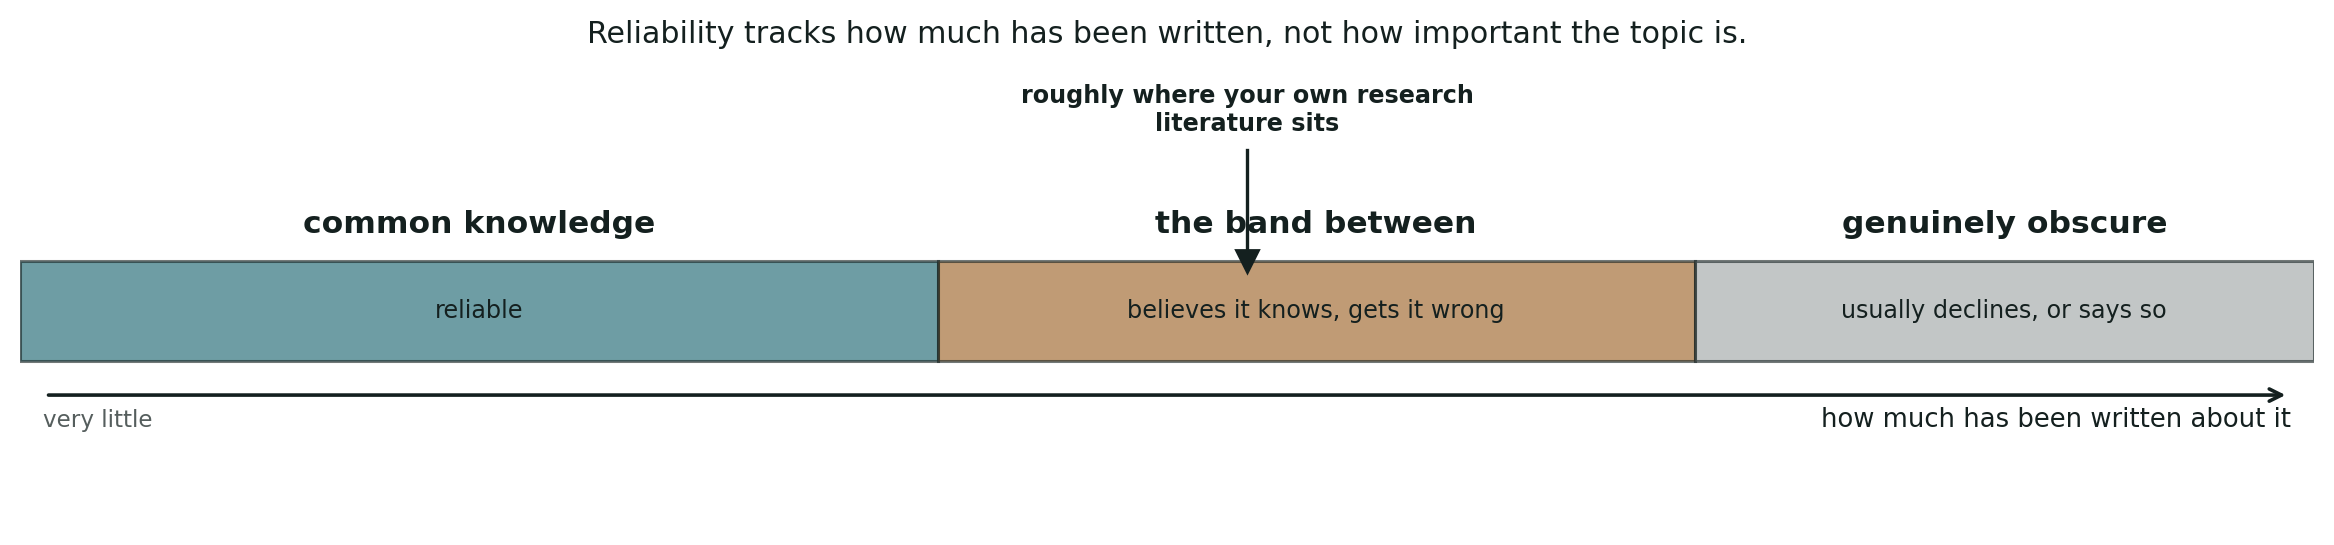
\includegraphics[height=34mm,width=\linewidth,keepaspectratio]{01-corpus-density}\end{center}
  {\small Contributors are instructed to build tasks in the middle band --- not common knowledge,
   where the model is reliable; not genuinely obscure, where it declines. \kw{That band is where
   your own literature sits.}}
  \provenance[One of five documents, stated as an operational rule.]{instrument}
\end{frame}
\note{%
The single most useful frame in this chapter for the room's own work, and the reason their
experience of the tool is what it is.\\[0.3em]
It explains why the tool feels reliable on textbook material and erratic on their research. The band
is not stumbled into; it is hunted.\\[0.3em]
The same figure appears in Chapter 1 and in Chapter 5, deliberately. It is the same fact seen three
times: as a property of the corpus, as a target of the rating pipeline, and as the shape of the
failure mode.\\[0.3em]
One document. Say so.}

% ---------------------------------------------------------------- 26
\begin{frame}{Attribution goes wrong: a phrasing found by search, given a story afterwards}
  \begin{center}
  \begin{tikzpicture}[node distance=7mm]
    \node[uhwide, text width=30mm]              (s) {an automated search\\over candidate\\instructions};
    \node[uhhi, right=of s, text width=28mm]    (b) {one phrasing\\scores best};
    \node[uhamber, right=of b, text width=30mm] (n) {it looks like\\encouragement};
    \node[uhghost, right=of n, text width=28mm] (e) {a story about\\why, invented\\afterwards};
    \draw[uhar] (s)--(b); \draw[uhar] (b)--(n); \draw[uhardot] (n)--(e);
  \end{tikzpicture}
  \end{center}
  {\small Reported gains up to 8\% and up to 50\% on two benchmarks, scored on one model. The
   winning instruction is specific to the model it was scored on; change the model and the best
   phrasing changes with it.}
  \citesource{yang2023,ye2024}
\end{frame}
\note{%
The first of two frames showing what happens when a behaviour is attributed to training and the
attribution is wrong. Say that is what they are for --- otherwise they read as digressions.\\[0.3em]
It was found by search, not by testing a hypothesis about encouragement. The narrative arrived
afterwards and it is the narrative that spread.\\[0.3em]
What this course will not claim: an earlier draft said later evaluations found the phrase does not
transfer to newer models. No primary re-evaluation could be found saying that. What is evidenced is
that optimised prompts do not transfer consistently across models, which is a different and
narrower claim.}

% ---------------------------------------------------------------- 27
\begin{frame}{Attribution goes wrong: the best of eleven, reported as the result}
  \begin{center}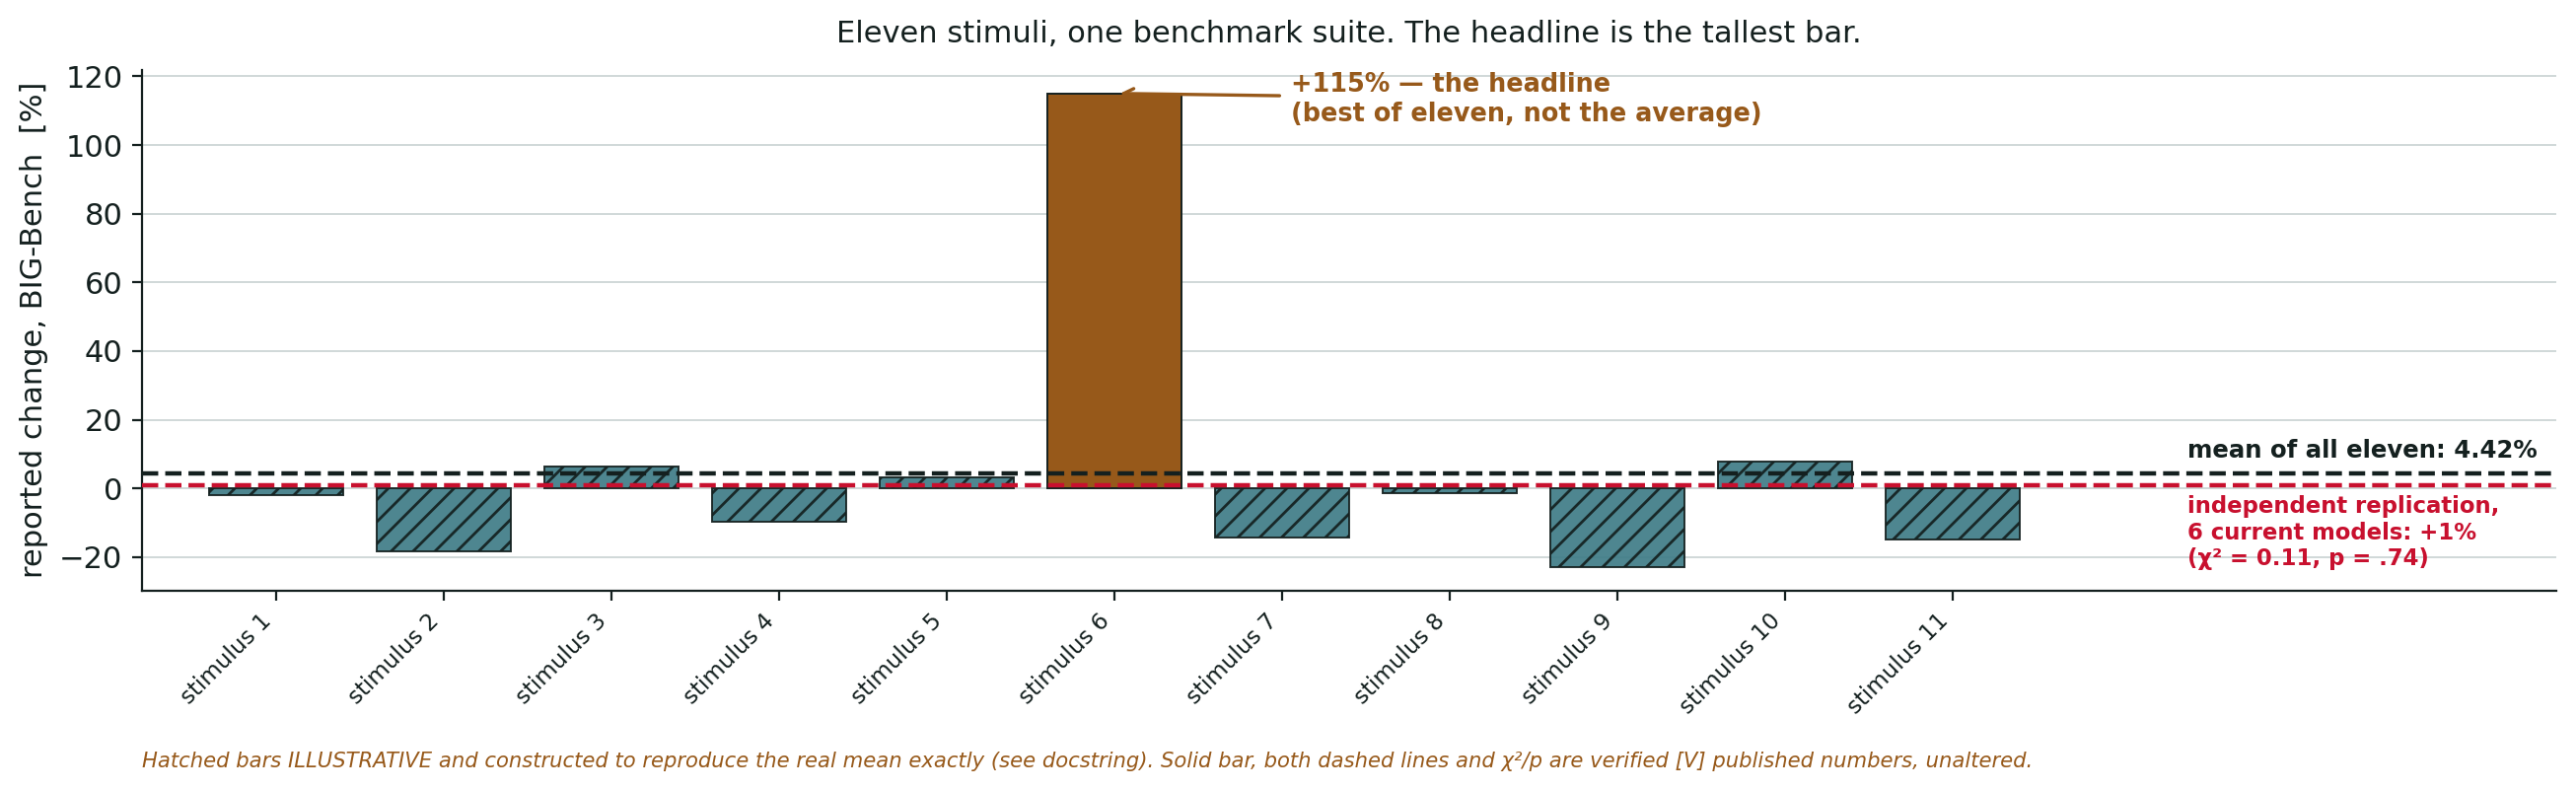
\includegraphics[height=31mm,width=\linewidth,keepaspectratio]{02-best-of-eleven}\end{center}
  {\small An independent replication across six current models found an insignificant increase of
   1\%. Re-deriving the original's own arithmetic gives \textbf{4.42\%} averaged over all eleven
   stimuli, against the \textbf{115\%} that became the headline.}
  \citesource{li2023emotion,vaugrante2024}
\end{frame}
\note{%
The sharpest quantitative moment in the chapter, and the one this room will feel in their own
work.\\[0.3em]
Point at the negative bars, because they are the part nobody expects. Given a maximum of 115\% and
a mean of 4.42\% over eleven, the other ten are forced to sum to $-66.4$\%. Most of the eleven
stimuli made performance \emph{worse}. That is not an embellishment in the figure; it is arithmetic
the two published numbers already require, and the figure asserts it in code rather than claiming
it in a caption.\\[0.3em]
The original is a technical report, not a peer-reviewed paper. The replicators' words: the numerical
values communicated in the study itself do not coincide with these claims.\\[0.3em]
The replicators' own limits belong beside their result. They did not use identical tasks or models,
wording varied, they sampled one stimulus per task by seed rather than reproducing the
best-of-eleven protocol, and they dropped one stimulus because models answered it instead of the
task. That third point matters most: the 1\% comes from a design that deliberately did not run
best-of-eleven, which is why the two numbers are not in contradiction.\\[0.3em]
Then the sentence that hands off: the same trap is available to anyone running five test cases and
reporting the best one.}

% ---------------------------------------------------------------- 28
\begin{frame}{The order used here is by evidence, and it is deliberately not the order of interest}
  \begin{center}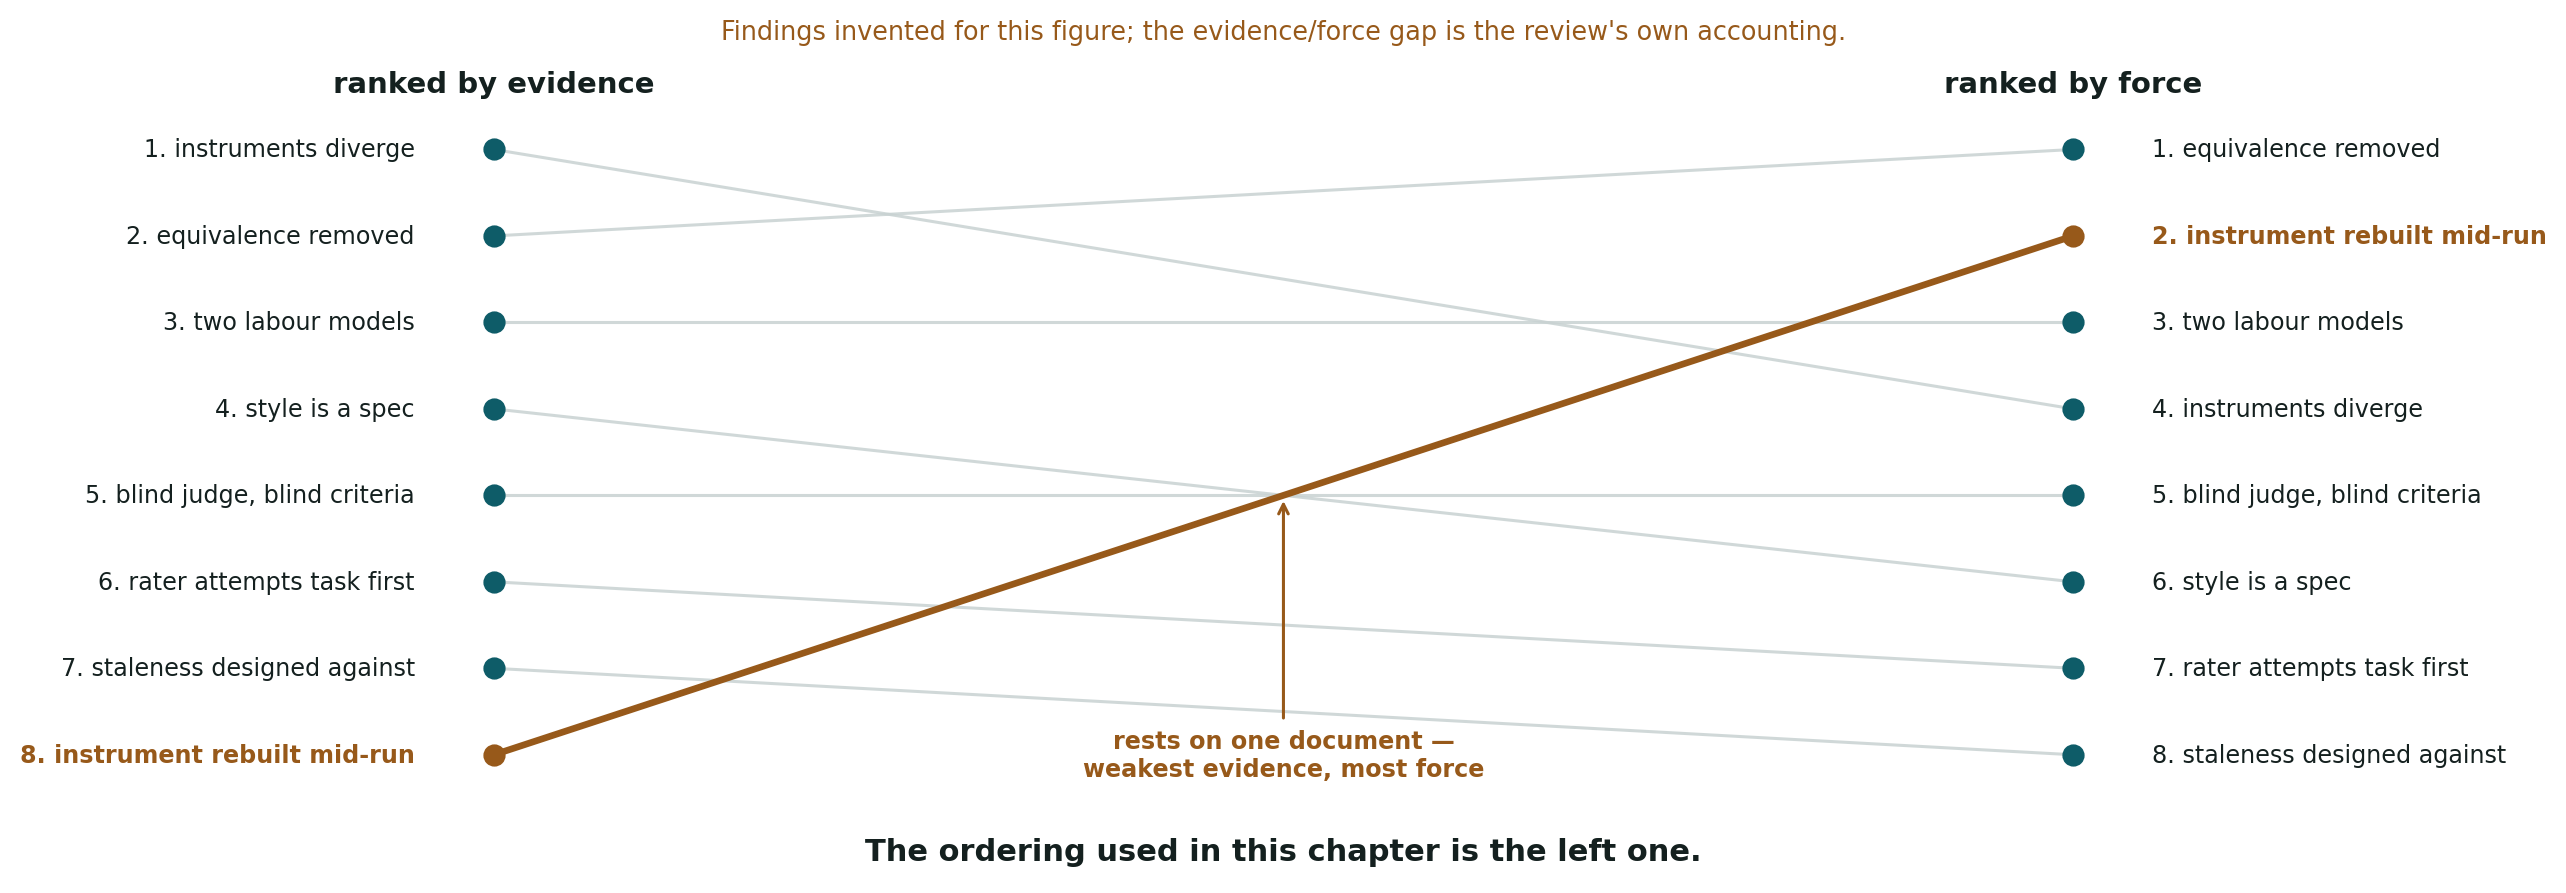
\includegraphics[height=33mm,width=\linewidth,keepaspectratio]{02-evidence-vs-force}\end{center}
  {\small The finding this room is most likely to remember --- an instrument rebuilt mid-collection
   --- ranks eighth. It rests on one changelog. Both of those are true at once, and printing the
   count on every frame is what lets you hold them together.}
  \provenance[The ranking is the instructor's, applied to fourteen findings.]{derived}
\end{frame}
\note{%
Saying this out loud is the point of the segment, and it is the frame that licenses everything
before it.\\[0.3em]
Two findings that made better stories in an earlier draft were demoted when further documents failed
to corroborate them. One was killed outright, and it is on the next frame.\\[0.3em]
The room is about to be asked to rate things, and the pressure they will feel in the exercise --- to
grade what is vivid rather than what is checkable --- is exactly the pressure this ordering resists.}

% ---------------------------------------------------------------- 29
\begin{frame}{What I got wrong while assembling this chapter}
  \vspace{0.5mm}
  {\footnotesize
  \begin{tabular}{p{0.40\linewidth} p{0.52\linewidth}}
    \textbf{The claim} & \textbf{What killed it} \\[0.4em]
    \hline \\[-0.6em]
    The rater's role migrates over time, from judge toward author
      & the earliest dated document already does both, and the only before-and-after evidence
        anywhere runs the other way \\[0.5em]
    Three features are how instruments work
      & each appeared in exactly one document of five \\[0.5em]
    The instruments share almost no vocabulary
      & too strong; two dimensions recur in three documents each \\[0.5em]
    The person's repaired text becomes training data
      & two claims welded together; the labour recurs, the collection does not \\
  \end{tabular}}
  \vspace{1.5mm}

  {\scriptsize The first survived two revisions before the evidence killed it, and it was the best
   story in the set.}
  \provenance[A correction log kept while the findings were assembled.]{derived}
\end{frame}
\note{%
Put this frame in front of a room of researchers and it does more for the chapter's credibility
than any of the surviving findings.\\[0.3em]
The first row is the one to dwell on. It was a clean narrative arc, it survived two revisions, and
it died because the earliest dated document already contained both behaviours and the single piece
of before-and-after evidence in the whole set pointed the other way. The correction removed the very
thing that made it a good story.\\[0.3em]
Say why the log exists: five documents from unknown vendors serving unknown clients cannot support
a claim about change over time, however many more are added. A time series needs the same vendor and
the same client at two moments.\\[0.3em]
Chapter 17 asks them to apply the same habit to their own arguments.}

% ---------------------------------------------------------------- 29
\begin{frame}{Now you do it}
  \begin{center}
  \begin{tikzpicture}[node distance=7mm]
    \node[uhwide, text width=30mm]              (a) {two responses to\\one request};
    \node[uhamber, right=of a, text width=26mm] (b) {one instrument};
    \node[uhhi, right=of b, text width=30mm]    (c) {eight minutes,\\visible time pressure};
    \draw[uhar] (a)--(b); \draw[uhar] (b)--(c);
  \end{tikzpicture}
  \end{center}
  \begin{columns}[t]
    \begin{column}{0.31\linewidth}\centering
      \kw{Your domain}\\[0.2em]{\small mechanics, concrete or fluids, so every one of you can check the physics}
    \end{column}
    \begin{column}{0.31\linewidth}\centering
      \kw{Record confidence}\\[0.2em]{\small a score per dimension, a preference, and how sure you are}
    \end{column}
    \begin{column}{0.31\linewidth}\centering
      \kw{Time-box the checking}\\[0.2em]{\small over two minutes to verify, mark it \textbf{unassessable}}
    \end{column}
  \end{columns}
  \provenance[The instrument is synthetic, built for this course on this room's domain.]{instrument}
\end{frame}
\note{%
The centrepiece. Say nothing about the expected outcome before the reveal --- announcing it would
void the demonstration the chapter is built on.\\[0.3em]
No preference is allowed unless the rater names a specific failure. That rule is what stops the
exercise becoming a vote on which response reads better.\\[0.3em]
Both responses are written from scratch for this course, on the shared domain. Nothing is borrowed
from any source document, and the rubric is synthetic.\\[0.3em]
Full specification in assets/rating-exercise/README.md.}

% ---------------------------------------------------------------- 30
\begin{frame}{How the session runs}
  \vspace{1mm}
  {\small
  \begin{tabular}{p{0.05\linewidth} p{0.62\linewidth} p{0.18\linewidth}}
    & \textbf{Step} & \textbf{Minutes} \\[0.3em]
    \hline \\[-0.6em]
    1 & \textbf{Rate}, individually, in silence, under visible time pressure & 8 \\[0.35em]
    2 & \textbf{Collect the tally} --- preference, then confidence beside it & 3 \\[0.35em]
    3 & \textbf{Reveal} the physical error and the fabricated citation & 5 \\[0.35em]
    4 & \textbf{Name what happened} & 5 \\[0.35em]
    5 & \textbf{Reviewer round} --- swap sheets, audit against the instrument & 10 \\[0.35em]
    6 & \textbf{Adjudicate} --- the defensible grade per axis, including where the rubric is ambiguous & 4 \\
  \end{tabular}}
  \vspace{2mm}

  {\scriptsize Steps 1 to 4 carry the lesson. With an odd number in the room, make one group of
   three at step 5 and rotate rather than swap.}
  \provenance{none}
\end{frame}
\note{%
If anything has to be cut, cut step 5 before anything else.\\[0.3em]
Say nothing about the expected outcome before step 3.\\[0.3em]
The minutes here are the exercise's internal pacing, not a claim about the chapter.}

% ---------------------------------------------------------------- 31
\begin{frame}{What to say after the reveal}
  \begin{center}
  \begin{tikzpicture}[node distance=6mm]
    \node[uhwide, text width=32mm]                (t) {read the tally back};
    \node[uhamber, right=of t, text width=34mm]   (c) {put confidence beside\\preference};
    \node[uhhi, right=of c, text width=36mm]      (u) {ask who marked the\\citation \textbf{unassessable}};
    \draw[uhar] (t)--(c); \draw[uhar] (c)--(u);
  \end{tikzpicture}
  \end{center}
  {\small Whatever the tally says, \kw{call it a tally}. Five or six raters is not a distribution,
   and this course does not present six points as one.}
  \provenance{derived}
\end{frame}
\note{%
Marking a fabricated citation unassessable rather than false is the correct action under the
instrument, and it is exactly how a fabricated citation passes into a dataset as acceptable. That
is the sentence the exercise exists to earn.\\[0.3em]
Then, and only here, the line the chapter has been building toward --- say it once, do not print it:
whatever preference this room just expressed, at scale that preference is a reward signal. They have
spent eight minutes generating training data.\\[0.3em]
If confidence and preference track each other, say so. The interesting version is not guaranteed to
happen, and claiming it did when it did not would be the failure this whole chapter warns about.\\[0.3em]
Then leave the question open: how many raters would we have needed before that tally meant anything?
Nobody here knows yet.}

% ---------------------------------------------------------------- 32
\begin{frame}{What we covered, and what is still open}
  \begin{columns}[t]
    \begin{column}{0.49\linewidth}
      {\usebeamercolor[fg]{frametitle}\bfseries What we covered}\\[0.5em]
      {\scriptsize
      \begin{itemize}\itemsep0.2em
        \item A predictor, plus demonstrations, plus preferences, plus optimisation against a
              model of those preferences
        \item The rating layer is smaller and more variable than \emph{human preferences} suggests
        \item Behaviour traces to mechanism, and the traces are not equally strong
        \item An instrument that cannot record a tie produces a dataset without ties
        \item Where a machine grades, criteria are stripped to the observable surface
      \end{itemize}}
    \end{column}
    \begin{column}{0.49\linewidth}
      {\usebeamercolor[fg]{frametitle}\bfseries What is still open}\\[0.5em]
      {\scriptsize
      \begin{itemize}\itemsep0.2em
        \item If instructions shaped it, which instructions steer it, and why those?
        \item How would you know a prompt change helped, rather than looked like it helped?
        \item How many raters would that tally have needed before it meant anything?
        \item Which behaviours on the mechanism table would survive better evidence?
      \end{itemize}}
    \end{column}
  \end{columns}
  \provenance{derived}
\end{frame}
\note{%
The takeaway for anyone attending only this session.\\[0.3em]
The open questions are the handoff. The first is Chapter 3, the second and third are Chapter 4, the
fourth is honest about the limits of what this chapter established. Do not print the chapter
numbers; say them if asked.\\[0.3em]
Five findings were held back and sit in the facilitator notes as answers to questions that will get
asked: score-and-rationale mismatch, the Goodhart machinery, execution as ground truth, minimum
citation counts, and role variation by client. Each rests on one document.}

\end{document}
